\documentclass[paper=A4,abstracton,twoside,openright,11pt,headsepline,BCOR=1cm,DIV=10,utf8]{scrreprt}

% do this first, since title of thesis might contain umlauts
\usepackage[utf8]{inputenc}

% TODO: fill in the information
\newcommand{\englishtitle}{Development of a framework for automated architecture validation}
\newcommand{\germantitle}{Entwicklung eines Frameworks für die automatisierte Architekturvalidierung}
\newcommand{\authorprename}{Rushanth}
\newcommand{\authorsurname}{Rasaratnam}
\newcommand{\matriculationnumber}{367117}
\newcommand{\examinors}{
	% Prüfer
	Prof. Dr.-Ing. Stefan Kowalewski\\
	Prof. Dr.\,rer.\,nat. Bernhard Rumpe
}
\newcommand{\advisors}{
	% Betreuer
	David Klüner M.Sc. \\
}


% import the preamble (manages all other imported packages)
% TODO: enable/disable specifics for theses written in german
% TODO: enable/disable BA (bachelor thesis) as thesis type
\usepackage[DE=true, BA=true]{preamble}

% Note: if you switch between different languages after the file has been compiled, it might be necessary to create the pdf multiple times to get rid of errors indicating that you havent loaded the package ngerman yet

% !TEX root = ../main.tex

% this file is read before \begin{document}

\DeclareMathOperator{\u8}{u8}
\DeclareMathOperator{\msb}{msb}    % import commands from file

%Abkürzungen:
%Abkürzungen:
\newacronym{i11}{I11}{Lehrstuhl Informatik 11}
\newacronym{RWTH}{RWTH}{Rheinisch-Westfälische Technische Hochschule Aachen}

\newacronym{asoa}{ASOA}{Automotive Service-oriented Architecture}
\newacronym[shortplural={E/E-Architekturen},longplural=elektrische/elektronische Architekturen]{eea}{E/E-Architektur}{elektrische/elektronische Architektur}
\newacronym{ecu}{ECU}{Electronic Control Unit}
\newacronym{can}{CAN}{Controller Area Network}
\newacronym{lin}{LIN}{Local Interconnect Network}
\newacronym{ivn}{IVN}{In-Vehicle Network}
\newacronym{dcu}{DCU}{Domain Control Unit}
\newacronym{zsu}{ZCU}{Zone Control Unit}
\newacronym{rest}{REST}{Representational State Transfer}
\newacronym{poc}{PoC}{Proof of Concept}
\newacronym{gui}{GUI}{Graphical User Interface}
\newacronym{api}{API}{Application Programming Interface}
\newacronym{qos}{QoS}{Quality-of-Service}
\newacronym{mbse}{MBSE}{modellbasierte Systementwicklung}
\newacronym{sdv}{SDV}{Software-Defined Vehicle}
\newacronym{autosar}{AUTOSAR}{AUTomotive Open System ARchitecture}
\newacronym[,longplural=Service-orientierte Architekturen]{soa}{SOA}{Service-orientierte Architektur}


%Symbole:
%Symbole
\newglossaryentry{symbol:V}{
	name=\ensuremath{V},
	description={Volumen [l]},
	sort=symbolV,type=symbolslist,
}
\newglossaryentry{symbol:pi}{
	name=\ensuremath{\pi},
	description={Kreiszahl [einheitenlos]},
	sort=symbolpi,type=symbolslist,
}

% --------------------------------------preambles-end-----------------------------------------

% Begin of the actual document
\begin{document}
\pagenumbering{Roman}
%\input{tex/commands2.tex}

% User specific options how latex shall split words at the end of a text line
% in case there is not enough space to fit the word. The listed word will be 
% split at the positions marked with -
% The list of words to split 
\hyphenation{
Byte-array
Si-mu-la-tion
Con-straint Con-straints Compare-Con-straints Bit-Mask-Con-straints
}

\pagestyle{scrheadings}

% do not modify the titlepage!
%% !TEX root = ../main.tex
% adapts automatically according to the selected language (for the preamble)
\titlehead{

\begin{textblock}{120}(85,0)
	
\includegraphics[height=3.1cm]{i11_Vector_RGB.pdf}
\end{textblock}
}

\ifthenelse{\boolean{ba}}{
	\newcommand{\thesistypeen}{Bachelor~Thesis}
	\newcommand{\thesistypede}{Bachelorarbeit}
	}{
	\newcommand{\thesistypeen}{Master~Thesis}
	\newcommand{\thesistypede}{Masterarbeit}
	}

  
\ifthenelse{\boolean{german}}{
	\subject{\thesistypede\\ 
	\vspace{0.15cm}\Large{\thesistypeen
	}}
}{
	\subject{\thesistypeen\\ 
	\vspace{0.15 cm}\Large{\thesistypede
	}}
}

\title{
\ifthenelse{\boolean{german}}{\germantitle}{\englishtitle}\\
\vspace{0.25cm}\vfil\Large{
\ifthenelse{\boolean{german}}{\englishtitle}{\germantitle}}
}
\author{\authorname\\
Matrikelnummer: \matriculationnumber}

\publishers{
\ifthenelse{\boolean{german}}{Gutachter}{Examiners}%
:\\ %research mentor
\examinors \\
\vspace{0.25cm}
\vfil
\vfil
\ifthenelse{\boolean{german}}{Betreuer}{Advisors}%
:\\
\advisors

\vfil
\vfil
\vspace{0.25cm}

\ifthenelse{\boolean{german}}{Diese Arbeit wurde vorgelegt am \\Lehrstuhl Informatik 11 -- Embedded Software}{This thesis was submitted to \\Lehrstuhl Informatik 11 -- Embedded Software}
}

\date{ Aachen, \today}



% dynamically set the thesis type according to the used language
\ifthenelse{\boolean{ba}}{
  \newcommand{\thesistypeen}{Bachelor~Thesis}
  \newcommand{\thesistypede}{Bachelorarbeit}
}{
  \newcommand{\thesistypeen}{Master~Thesis}
  \newcommand{\thesistypede}{Masterarbeit}
}

\ifthenelse{\boolean{german}}{

  \renewcommand{\subject}{\thesistypede\\
    \vspace{0.3cm}{\thesistypeen\\}}
}{
  \renewcommand{\subject}{\thesistypeen\\
    \vspace{0.3 cm}{\thesistypede\\}}
}

% set title page
\renewcommand*{\maketitle}{%
  \begin{titlepage}
    \begin{textblock}{120}(85,0)
      
\includegraphics[height=3.1cm]{i11_Vector_RGB.pdf}
    \end{textblock}

    % empty
    \
    \vspace{0.5cm}

    % thesis type
    \centering
    \textbf{\subject}

    \vspace{0.8cm}
    \vfill

    % thesis title		% TODO: größer & andere Schriftart
    \textbf{
      \LARGE{\ifthenelse{\boolean{german}}{\germantitle}{\englishtitle}}\\
      \vspace{0.3cm}
      \Large{\ifthenelse{\boolean{german}}{\englishtitle}{\germantitle}}\\
    }

    \vspace{0.8cm}
    \vfill

    % student
    \authorname\\
    Matrikelnummer: \matriculationnumber\\

    \vspace{0.3cm}
    \vfill

    % metainfo
    Aachen, \today
    \vspace{0.3cm}
    \vfill

    \ifthenelse{\boolean{german}}{Gutachter}{Examiners}%
    :\\ %research mentor
    \examinors \\
    \vspace{0.3cm}
    \vfil
    \ifthenelse{\boolean{german}}{Betreuer}{Advisors}%
    :\\
    \advisors

    \vspace{0.3cm}
    \vfill

    \ifthenelse{\boolean{german}}{Diese Arbeit wurde vorgelegt am \\Lehrstuhl Informatik 11 -- Embedded Software}{This thesis was submitted to \\Lehrstuhl Informatik 11 -- Embedded Software}



  \end{titlepage}
}

\maketitle

% OPTIONAL (remove if you don't want a dedication)
%% define basic appearence for dedication
\renewcommand{\dedication}{
	\cleardoublepage
	\thispagestyle{plain}
	\ \par
	\vspace{5cm}
	\noindent
	\ifthenelse{\boolean{german}}{\textbf{Dankeswort}}{\textbf{Acknowledgments}}
	\vspace{-0.5cm}
	\begin{flushleft}
		\noindent
	\end{flushleft}}

\dedication{
\ifthenelse{\boolean{german}}{
Vorab möchte ich mich bei einigen Personen bedanken, die mich bei der Erstellung dieser Arbeit unterstützt haben:
}{
Ex ante, I'd like to thank the listed persons below who supported me during the editing time of this thesis:
}
\begin{itemize}
	\item Person XY for ...,
	\item The coffee machine of i11.
\end{itemize}
}

%\listoftodos[This is to be done] 	% TODO: exclude in final version
% the list of todos should not be part of the final thesis and is only intended to show the advisor(s) of what flaws the student is already aware of)

% Abstract of the thesis
% !TEX root = ../main.tex
\begin{abstract}

  % Für deutschsprachige Ausarbeitungen sollte jeweils ein Abstract in deutscher und englischer Sprache verfasst werden
  % If written in german their should be two, a german and an english abstract


  % Kurze Motivation und Angabe was in der Arbeit behandelt wird. Dies wird in der Einleitung ausführlicher behandelt.
  % Brief motivation and explanation of the topic. This will typically be repeated more extensive in the "`introduction"' chapter.
  \noindent
  Die Automobilindustrie befindet sich im Wandel, wobei sich der Fokus auf die Entwicklung softwaredefinierter Fahrzeuge verlagert. Die daraus resultierende zunehmende Komplexität verteilter Systeme erfordert neue Ansätze für die Validierung in frühen Entwicklungsphasen. Ziel dieser Arbeit ist die Entwicklung eines Frameworks zur automatisierten Architekturvalidierung im bereits bestehenden ArchitekturTool des Projekts AUTOtech.agil, das zur Spezifikation von verteilten Systemen genutzt wird. Das entwickelnde Framework umfasst eine standardisierte API zur Anbindung beliebiger Algorithmen, eine Benutzeroberfläche zum Ausführen der angebundenen Algorithmen sowie eine Komponente zur Visualisierung der Ergebnisse. Als Proof of Concept wurde ein erster Validierungsalgorithmus implementiert, der einen Traceability-Check durchführt und die Nachverfolgbarkeit zwischen Anforderungen und Garantien prüft. Die Evaluation belegt, dass das Framework alle gesetzten funktionalen und nicht-funktionalen Anforderungen erfüllt und eine erweiterbare Grundlage für die automatisierte Architekturvalidierung in der Fahrzeugtechnik bietet.

\end{abstract}


\begin{otherlanguage}{english}
  \begin{abstract}
    The automotive industry is experiencing a change, with a shift in focus toward the development of software-defined vehicles. The resulting increase in complexity of distributed systems requires new approaches to validate within early development phases. The aim of this work is to develop a framework for automated architecture validation within the existing ArchitekturTool of the AUTOtech.agil project, which is used to specify distributed systems. The developed framework includes a standardized API for integrating any algorithms, a user interface for executing the integrated algorithms, and a component to visualise the results. As a proof of concept, a validation algorithm was implemented that runs a traceability check and verifies the link between requirements and guarantees. The evaluation shows that the framework meets all (non-)functional requirements and provieds an extendable basis for automated architecture validation within automotive engineering.
  \end{abstract}
\end{otherlanguage}

% Eidesstattliche Erklärung
% Note: there is an english translation available (eidesstattlicheVersicherungZPA_en.pdf). 
% However, the german version is legally binding and required to be a part of the thesis.
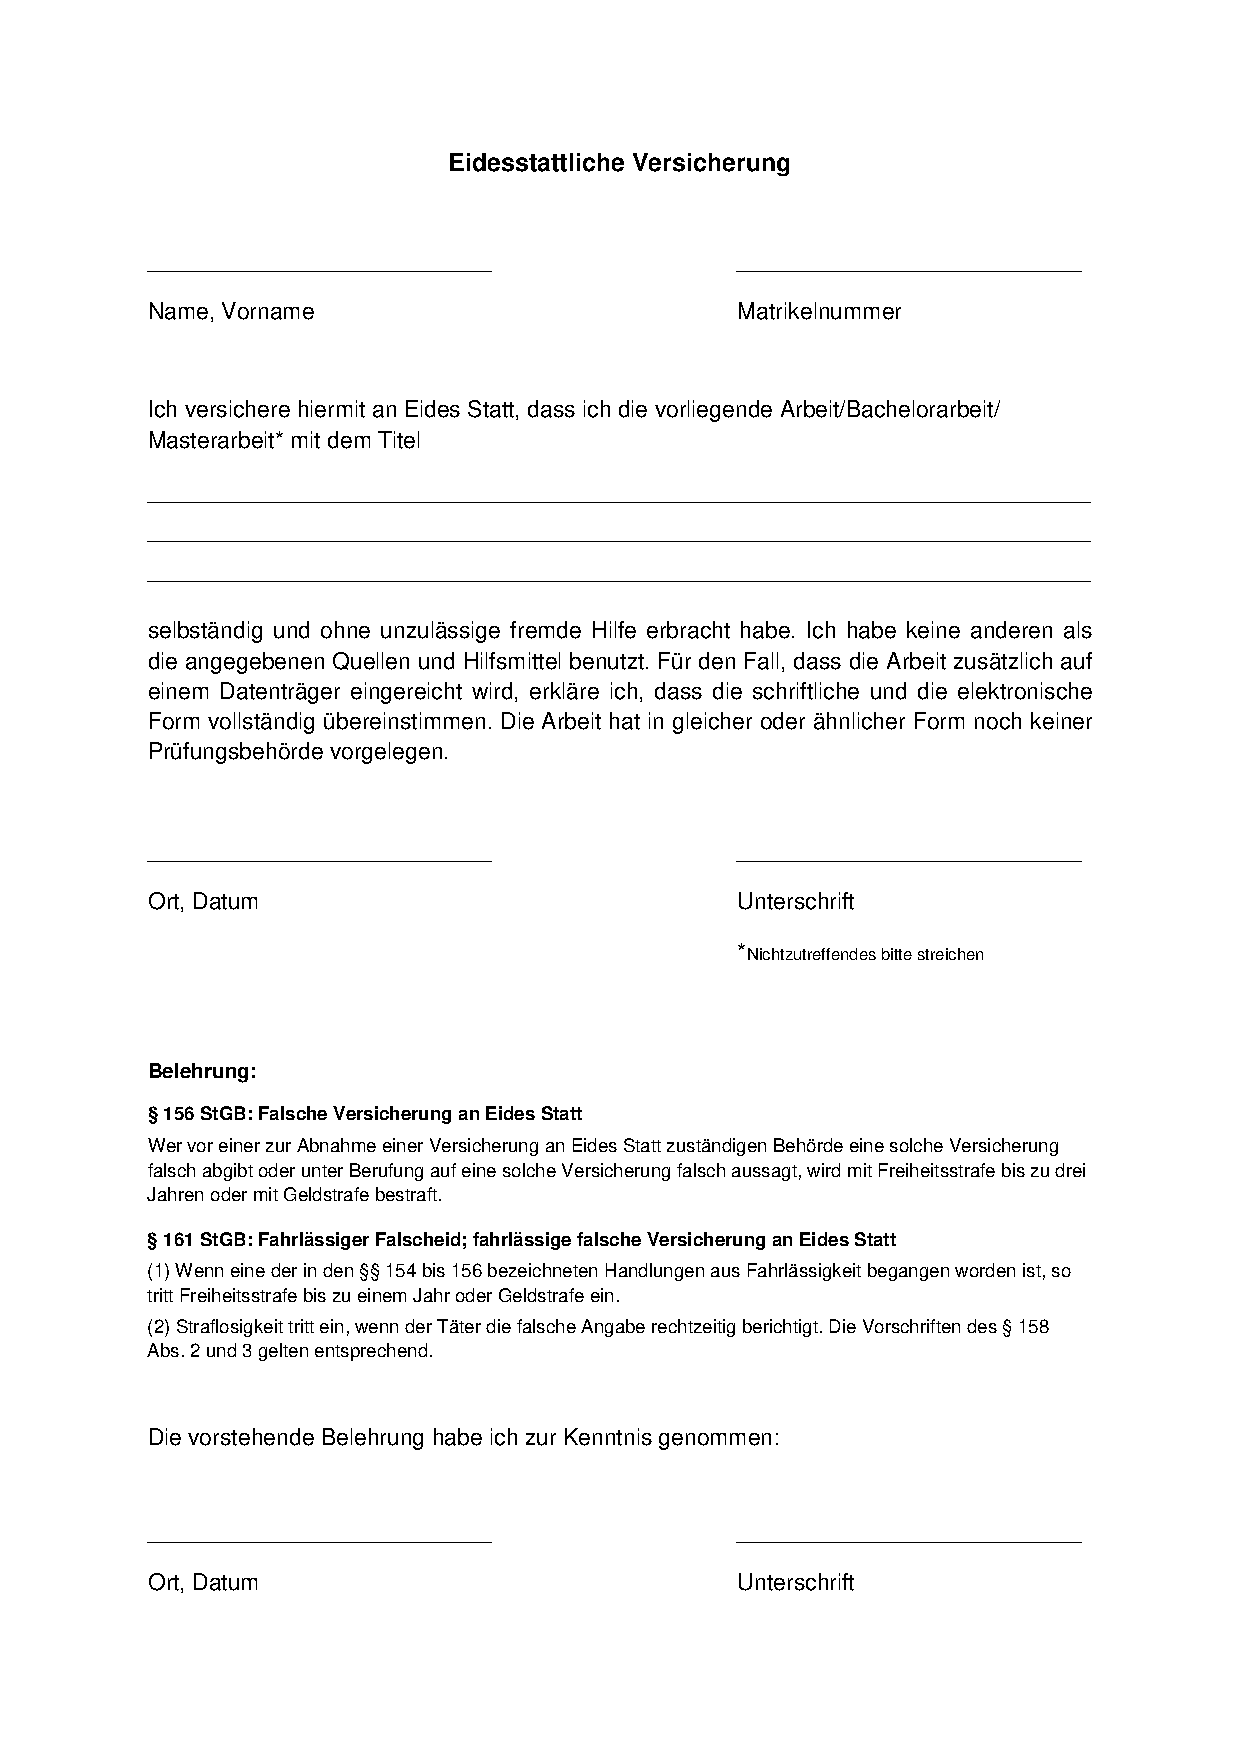
\includepdf[pages={1}]{eidesstattlicheVersicherungZPA.pdf}
% this page may not be manipulated

\newpage
\thispagestyle{empty}
\begin{center}
	\Large\textbf{Eidesstattliche Versicherung}
\end{center}
\vspace{5mm}

\begin{spacing}{0.4}
\noindent 
\begin{minipage}[t]{0.41\textwidth}
		\authorsurname,~\authorprename\\
		\noindent 
		\rule{\textwidth}{0.4pt} \\\\
		Name, Vorname
\end{minipage}
\hfill
\begin{minipage}[t]{0.41\textwidth}
	\matriculationnumber\\
	\noindent 
	\rule{\textwidth}{0.4pt}\\\\
	Matrikelnummer
\end{minipage}
\end{spacing}


\vspace{10mm}
\noindent
Ich versichere hiermit an Eides Statt, dass ich die vorliegende \ifthenelse{\boolean{ba}}{Bachelorarbeit}{Masterarbeit} mit dem Titel
\vspace{4mm}

\noindent
\textbf{\germantitle}


\vspace{4mm}
\noindent
selbständig und ohne unzulässige fremde Hilfe erbracht habe. Ich habe keine anderen als die angegebenen Quellen und Hilfsmittel benutzt. Für den Fall, dass die Arbeit zusätzlich auf einem Datenträger eingereicht wird, erkläre ich, dass die schriftliche und die elektronische Form vollständig übereinstimmen. Die Arbeit hat in gleicher oder ähnlicher Form noch keiner Prüfungsbehörde vorgelegen.\\
\vspace{4mm}
\vfil

\begin{spacing}{0.4}
\noindent 
\begin{minipage}[t]{0.41\textwidth}
	\rule{\textwidth}{0.4pt}\\\\
	Ort, Datum
\end{minipage}
\hfill
\begin{minipage}[t]{0.41\textwidth}
	\rule{\textwidth}{0.4pt}\\\\
	Unterschrift
\end{minipage}
\end{spacing}

\vfill
%\vspace{14mm}
\noindent
\textbf{Belehrung:}

\vspace{4mm}
\vfil
\noindent
\textbf{\S~156 StGB: Falsche Versicherung an Eides Statt}\\
Wer vor einer zur Abnahme einer Versicherung an Eides Statt zuständigen Behörde eine solche Versicherung
falsch abgibt oder unter Berufung auf eine solche Versicherung falsch aussagt, wird mit Freiheitsstrafe bis zu drei
Jahren oder mit Geldstrafe bestraft.\\


\noindent
\textbf{\S~161 StGB: Fahrlässiger Falscheid; fahrlässige falsche Versicherung an Eides Statt}\\
(1) Wenn eine der in den §§ 154 bis 156 bezeichneten Handlungen aus Fahrlässigkeit begangen worden ist, so
tritt Freiheitsstrafe bis zu einem Jahr oder Geldstrafe ein.\\
(2) Straflosigkeit tritt ein, wenn der Täter die falsche Angabe rechtzeitig berichtigt. Die Vorschriften des § 158
Abs. 2 und 3 gelten entsprechend.\\


\noindent
\normalsize Die vorstehende Belehrung habe ich zur Kenntnis genommen:\\
\vspace{4mm}
\vfil

\begin{spacing}{0.4}
	\noindent 
	\begin{minipage}[t]{0.41\textwidth}
		\rule{\textwidth}{0.4pt}\\\\
		Ort, Datum
	\end{minipage}
	\hfill
	\begin{minipage}[t]{0.41\textwidth}
		\rule{\textwidth}{0.4pt}\\\\
		Unterschrift
	\end{minipage}
\end{spacing}


% TODO: remove/add % symbols before the required rows
\tableofcontents  % Inhaltsverzeichnis
\listoftables		% Tabellenverzeichnis
\listoffigures   % Abbildungsverzeichnis

% TODO: see http://texblog.org/2014/01/15/glossary-and-list-of-acronyms-with-latex/ 
% at Capitalize and pluralize terms for a brief introduction on how to use acronyms 

% print acronym list
\ifthenelse{\boolean{german}}{
  \printglossary[type=\acronymtype,style=long, title=Abkürzungsverzeichnis] % use this for german version
}{
  \printglossary[type=\acronymtype,style=long, title=List of Acronyms]
}

% print symbol list
\ifthenelse{\boolean{german}}{
  \printglossary[type=symbolslist,style=long, title=Symbolverzeichnis] % use this for german version
}{
  \printglossary[type=symbolslist,style=long, title=List of Symbols]
}

\pagestyle{scrheadings}

% TODO: write your content into the chapters
\cleardoublepage\pagenumbering{arabic}
% !TEX root = ../main.tex

\chapter{Einleitung}
\label{ch:introduction}
Die Automobilindustrie befindet sich im Wandel, der sich durch den Fokus weg vom mechanikzentrierten Fahrzeug hin zum \gls{sdv} zeigt. Während früher die mechanischen Komponenten ausschlaggebend waren für den Verkauf eines Fahrzeuges, rückt heute die Software immer mehr in den Fokus und wird zum zentralen Differenzierungsmerkmal moderner Fahrzeuge \cite{Cha21}\cite{zhao2022}.

Der Fokus auf \gls{sdv} geht mit der deutlich steigenden Komplexität von \glspl{eea} einher \cite{Cha21}\cite{Pancik2018}. Moderne Fahrzeuge enthalten oft über ein hundert \glspl{ecu}, umfangreiche Verkabelung und Millionen Zeilen von Code. Diese komplexen Architekturen müssen sorgfältig geprüft werden. Da eine späte Fehlererkennung zu erheblichen Kosten führt, sollte dies bereits in frühen Entwicklungsphasen passieren \cite{Cha21}.

Für die Modellierung und Entwicklung dieser Architekturen existieren bereits funktionsfähige, jedoch meist kostenpflichtige Tools wie PREEvision, die als Industriestandard gelten. Allerdings sind fast alle dieser Tools nicht open-source und bieten nicht alle möglichen Validierungsarten an um die verteilten Systeme auf Herz und Niere zu prüfen \cite{askaripoor2022architecture}\cite{schauffele2016architectural}.

Hier setzt das \textit{AUTOtech.agil}-Projekt\footnote{https://www.autotechagil.de/} an. Ziel des Projekts ist die Entwicklung einer offenen Software- und \gls{eea} für zukünftige Fahrzeuggenerationen \cite{autotechagil2024}\cite{vanKempen2023}. Neben der Service-orientierten Architektur ASOA\footnote{\gls{asoa}} wurde auch ein webbasiertes Tool zur Spezifikation von funktionalen, Softwarebezogenen und \gls{eea} geforscht. Dieses Tool, das \textit{ArichtekturTool},  soll eine open-source und zukunftsfähige Alternative zu den bestehenden Industriestandards sein.

Jedoch fehlt diesem Tool noch eine Funktion zur automatisierten Architekurvalidierung. Genau hier liegt der Beitrag der vorliegenden Abschlussarbeit: Das ArchitekturTool um eine automatisierte Validierungsfunktion zu erweitern, um dem Endutzer beim Entwicklungsprozess zu unterstützen.
\section{Aufgabenstellung}
\label{sect:aufgabenstellung}

Das Ziel dieser Arbeit ist das ArchitekturTool um die folgenden Funktionalitäten zu erweitern, um eine automatisierte Architekturvalidierung zu ermöglichen. Dazu wird zunächst eine \gls{api} zur Anbindung von Validierungsalgorithmen entwickelt. Anschließend wird eine \gls{gui} umgesetzt, mit der die hinterlegten Validierungsalgorithmen ausgeführt werden können. Zur Analyse beziehungsweise Interpretation der Ergebnis wird zudem eine entsprechende \gls{gui} für die Ergebnisse dieser Algorithmen implementiert. Abschließend wird ein erster Validierungsalgorithmus in die neu entwickelte Umgebung zu hinzuzufügt.
\section{Aufbau der Arbeit}
\label{sec:aufbau}

Der Aufbau dieser Arbeit ist wie folgt: Zunächst werden im Kapitel~\ref{ch:basics} die notwendigen Grundlagen zum Verständnis der Arbeit behandelt. Dazu gehören eine kurze Einführung in das ArchitekturTool, die Erläuterung der \gls{eea} im Bereich der Automobilindustrie sowie ein Überblick über die relevanten Konzepte, wie \gls{soa} und Middleware innerhalb eines Fahrzeuges. Des Weiteren werden die Motivation und Methoden hinter der Architekturvalidierung sowie der bestehende Webentwicklungs-Stack vorgestellt.

Anschließend wird in Kapitel~\ref{ch:relatedWork} der Stand der Technik betrachtet. Hier werden die in der Industrie verbreiteten Tools und Plattformen zur Architekturmodellierung und -validierung wie PREEvision, Simulink + System Composer und Capella im Detail vorgestellt und im Hinblick auf ihren Validierungsfunktionen verglichen. Abschließend werden die verschiedenen Ansätze zur Architekturvalidierung betrachtet.

In Kapitel~\ref{ch:KuD} folgt das Konzept und Design des im Rahmen dieser Arbeit entwickelten Frameworks. Ausgehend von einer Anforderungsanalyse werden der Entwurf der Validierungs-Engine, die Systemarchitektur sowie das Konzept der \gls{api} und der \gls{gui} erläutert.

Danach wird in Kapitel~\ref{ch:imp} die praktische Umsetzung beschrieben. Dabei wird sowohl die Backend-Implementierung der Algorithmenverwaltung und Validierungs-Engine, als auch die Realisierung der Frontend-Komponenten erläutert. Außerdem wird der erste Validierungsalgorithmus als \gls{poc} vorgestellt.

In Kapitel~\ref{ch:evaluation} wird das entwickelte Framework evaluiert. Mithilfe des ersten Validierungsalgorithmus werden in einem Testszenario die wichtigsten Funktionen geprüft und die Ergebnisse bewertet.

Abschließend werden im \ref{ch:fazit}. Kapitel alle Erkenntnisse zusammengetragen und mit einem Ausblick auf mögliche Weiterentwicklungen hingewiesen.
% !TEX root = ../main.tex
%\chapter{Background}
\chapter{Grundlagen}
\label{sect:basics}

The chapter about the background should introduce all preliminary knowledge the reader should have before reading the part of the thesis where the actual contribution to a topic is presented.
Such preliminary knowledge could be theoretic aspects, domain knowledge or special notations being used, e.\,g., diagram types for visualization purpose.
Generally this chapter does not present any contributions of the author.
Thus, the background chapter makes often extensive use of citations providing the information whose work is presented.
In case the background chapter presents nonetheless work of the thesis author, make sure that this is absolutely clear.

% Jedes Kapitel/Abschnitt sollte mit einem (zumindest kurzen) einführenden Text beginnen der 
% erklärt worum es in diesem Kapitel geht (siehe About Chapters and Sections)
% Each chapter should start with an (short) introduction explaining what the chapter is about 
% (see About Chapters and Sections)



% Die Abschnitte des Grundlagenkapitels sind exemplarisch!
% The sections of the fundamentals chapter are only examples!



\section{About Chapters and Sections}
\label{sect:chaptsect}

At the beginning of each chapter or section the writer should introduce the reader to the specific (sub-)topic addressed.
This is intended to provide a continuous reading experience.
In a similar way, there should be some final words at the end of each chapter or section anticipating the next subtopic.
Of course, the chapters and sections have to be ordered such that there is a connection between them.
An outline about the different sections of a chapter shall be given at the beginning of each chapter, too.
Moreover, please ensure that different headings do not consecutively follow each other without text in between.
After this section has dealt with the connections between different chapters and sections, the next section explains some frequently used latex commands.

An example how this could look like for the beginning of the Background chapter which should have been written before this section is given below:\\
This chapter presents some latex fundamentals and is divided into two sections.
The first section \ref{sect:chaptsect} deals with the structuring of the text, namely introductions and connections between chapters and sections.
The second section \ref{sect:latex} presents some basic knowledge on setting up the latex environment to create this document and two latex commands which will be used.

% ----------------------------------------------------------------------------------------------------

\section{Latex-technicals}
\label{sect:latex}

This section intends to introduce the reader without or only few latex knowledge to some basic latex commands.
It starts with a short introduction on how to get started with Latex and the setup of a latex environment.
In order to explain some useful features for document creation, Sect.~\ref{sect:citations} presents a citation command and gives some instructions on \textit{bibtex}.
Consequently, Sect.~\ref{sect:illustrations} explains how illustrations can be added to a document\footnote{A brief explanation on how to use symbols and abbreviations with this template can be found in appendix \ref{app:c}}.

\subsection{Setting up the environment}
\label{sect:latexenvironment}
The creation of documents using Latex can be compared to the creation of programs using a programming language like C.
This means that the Latex source files are simple text files.
These files describe the document being constructed and can be \enquote{compiled} to generate the document.
Accordingly a latex compiler is required by the user to create documents.
The open source project MiKTeX\footnote{\url{http://miktex.org/about}} includes such compilers.
This software-package contains everything needed to create Latex files out of this template.
Please note, that it does not contain all required packages to compile this document.
However, it is possible to obtain the required packages during latex compilation automatically.
If this is not initially the case, the feature can be enabled by starting the configuration program located at \enquote{Miktex install directory/miktex/bin/x64/mo\_admin}.
The option is configurable under the general tab at the section \enquote{package installation}.
Depending on the enabled/used features (e.\,g., creation of index etc.) this document requires to be created with additional parameters what can easily be done using the \texttt{compile.bat} script, delivered with this template.

As for programming languages \textit{Integrated Development Environments} (IDE) can support the user during his work.
An example for such an IDE compatible with MiKTeX is TeXnicCenter.
The reader might want to take a look at the correspondent website \url{http://www.texniccenter.org/}.


Since it has been explained how a Latex environment can be set up the following two sections describe some basic commands which will be needed to create scientific documents.

\subsection{Citations}
\label{sect:citations}

Latex is widely used to write scientific papers or theses.
A general commonality of such documents is the need to refer to work provided by other parties.
To cope with this need latex provides in combination with bibtex\footnote{bibtex is used to generate the bibliography} the \textbackslash cite\{reference-tag\} command.
During the creation of a latex document occurrences of the \textbackslash cite\{\} command are automatically replaced with squared brackets and a generated tag in between.
Those tags are listed in the bibliography with information about author, publisher, etc. referring to the literature information was taken from.
For instance, the command \textbackslash cite\{columbia\} will be transformed during creation of this latex document into \cite{columbia}.
This transformation requires that there is a correspondent entry for the \enquote{columbia} reference-tag in the \enquote{references.bib} file which comes with this latex template\footnote{In case a web content is referenced, a timestamp indicating the content was consulted shall be part of the bibliography entry. 
Moreover, offline copies of the contents need to be provided. This ensures that readers will be able to understand your work in the future when cited web content may have changed or be unavailable.}.

The next latex feature introduced in this document is the possibility to use illustrations, which is the topic of the following section.

\subsection{Illustrations}
\label{sect:illustrations}

Latex documents may contain pictures to support and visualize explanations.
They can be added to a document using the following commands:

\begin{flushleft}

\textbackslash begin\{figure\} \\
	\textbackslash centering \\
		\textbackslash includegraphics\{path\_to\_picture\} \\
	\textbackslash caption\{This caption will be shown below the figure\} \\
	\textbackslash label\{fig:label\_to\_referrence\_the\_figure\} \\
\textbackslash end\{figure\} \\

\end{flushleft}


An example how this looks after creation of the document is shown in Fig.~\ref{fig:logo}.
\begin{figure}[H]
	\centering
		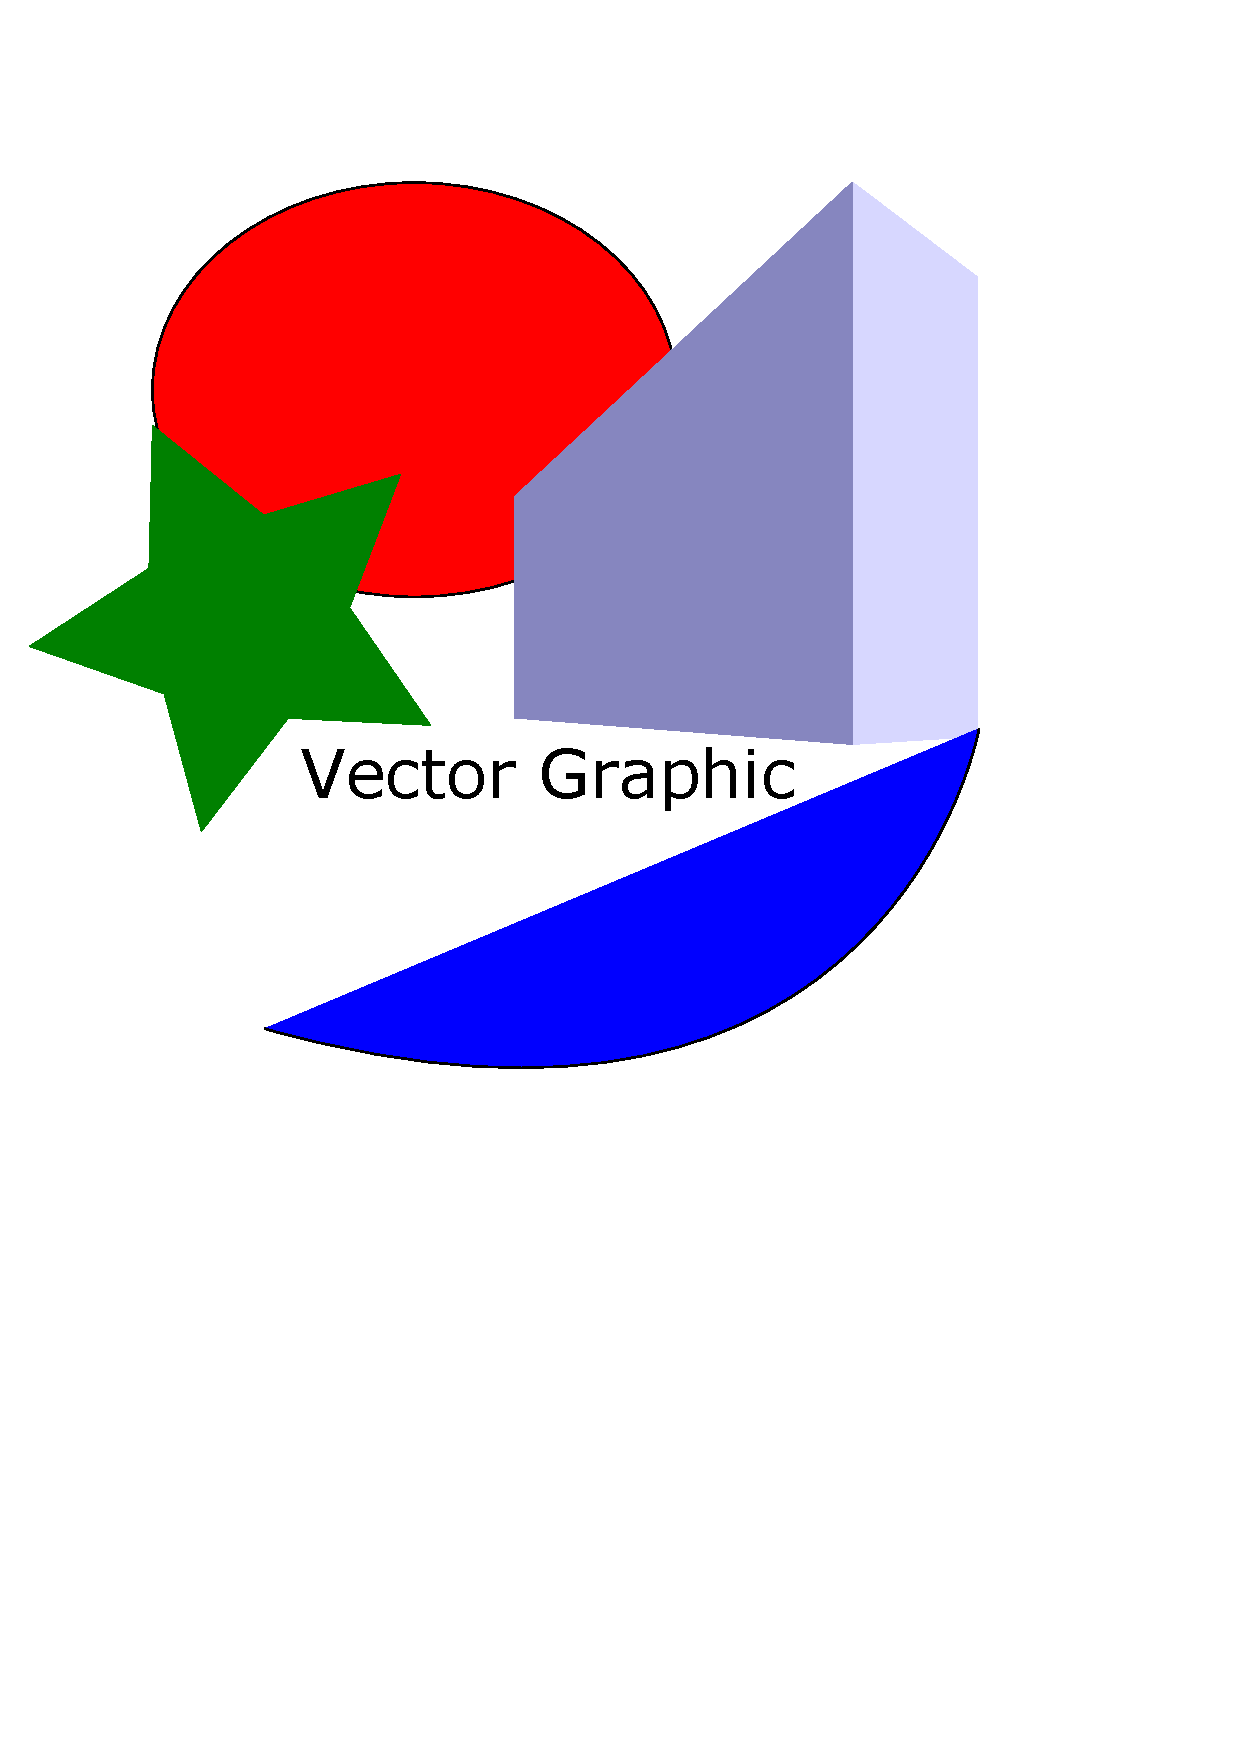
\includegraphics[width=0.40\textwidth]{figures/vectorGraphic.pdf}
	\caption{Example of a vector graphic}
	\label{fig:logo}
\end{figure}

Since this document is not the first and only one providing advice and hints regarding latex and structuring theses, the following chapter presents related work in this field.
% !TEX root = ../main.tex

\chapter{Stand der Technik}
%\chapter{Related Work}
\label{sect:relatedWork}

% Dieses Kapitel kann auch als Abschnitt im vorherigem Grundlagen Kapitel enthalten sein.
% Dies kann je nach Art der verwandten Arbeit und wie diese mit der aktuellen Arbeit verknüpft ist eine logischere Gliederung darstellen.
% This chapter can alternatively be a section of the background chapter. Depending on the relations between the actual and the related work,
% it can be a more intuitive, logic and consistent structuring to mention the related work in the previous chapter.

% Kurz vorstellen was es noch in dem Gebiet gibt und worin sich diese Arbeit davon unterscheidet
% Short presentation/summary of what has been done already in the research area and how it differs from the current thesis.
In diesem Kapitel werden die bestehenden Werkzeuge zum Spezifizieren von Architekturen im Bereich der Fahrzeugindustrie sowie die von ihnen verwendeten Verfahren zur Architekturvalidierung. Dies ermöglicht ein besseres Verständnis für den Beitrag, den die Abschlussarbeit leistet.

\section{Etablierte Werkzeuge und Plattformen}
Um die zunehmende Komplexität der \glspl{eea} in modernen Fahrzeugen mit Blick auf autonome Fahrfunktionen und Fahrassistenzsystemen zu bewältigen, wird aktiv an Software gearbeitet, die es Entwicklern und Ingenieuren ermöglicht, funktionale, softwarebezogene und \glspl{eea} zu modellieren bzw. zu spezifizieren \cite{askaripoor2022architecture} \cite{schauffele2016architectural}. Im folgenden werden die Werkzeuge PREEvision und Simulink + System Composer, welche als Industriestandard gelten, und Capella als kostenlose Alternative analysiert.


\subsection{Vector PREEvision}
PREEvision ist ein kommerzielles, modellbasiertes Werkzeug zur Entwicklung und Optimierung verteilter, eingebetteter Systeme in der Automobilindustrie. Das Hauptziel des Werkzeugs ist es, die zunehmende Komplexität der \glspl{eea} innerhalb der \glspl{sdv} beherrschbar zu halten \cite{askaripoor2022architecture}. Das  Werkzeug richtet sich dabei an die weit akzeptierten Automobilstandards wie \gls{autosar} RIF/ReqIF\footnote{Requirements Interchange Format: www.automotive-his.de/rif}, KBL\footnote{Kabelbaumliste: www.vda.de
} und VEC\footnote{Vehicle Electric Container: www.vda.de} \cite{schauffele2016architectural}. Es werden außerdem die drei System-Engineering-Prinzipien unterstützt: Abstraktion (Implementationsaspekte auf eine konzeptionellere Ebene abstrahieren), Dekomposition (System kann in jeder Schicht hierarchisch zerlegt werden), Wiederverwendung (Komponenten und Modelle können von verschiedensten Produktlinien und Varianten verwendet werden) \cite{schauffele2016architectural}.

\begin{figure}
  \centering
  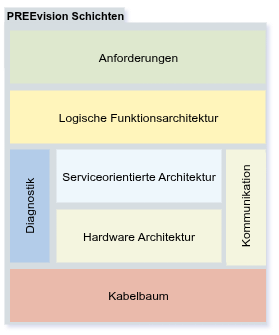
\includegraphics[width=0.5\textwidth]{figures/PREEVISION_LAYER.drawio.png}
  \caption{Schematische PREEvision Schichtenarchitektur. (Nachzeichnung von \cite{vectorinformatikgmbhpreevision})}
  \label{fig:preevision_schicht}
\end{figure}

Der Schwerpunkt von PREEvision ist jedoch, die auf Abbildung~\ref{fig:preevision_schicht} grob dargestellte Schichtenarchitektur.Die Abbildung zeigt den Weg von der abstrakten Anforderungsebene zur konkreten Implementierung. Ausgehend von den Anforderungen wird eine Logische Funktionsarchitektur entworfen, welche dann in eine \gls{soa} und eine Hardware Architektur überführt wird, bis hin zum physischen Kabelbaum. Dieser durchgängige Ansatz stellt sicher, dass alle Aspekte des Systems, inklusive Diagnostik und Kommunikation, miteinander verbunden sind (Single-Source-of-Truth) \cite{schauffele2016architectural}. Eine detaillierte Abbildung der Schichtenarchitektur ist im Appendix~\ref{appendix:preevision_layer_model} zu finden.


\subsection{Mathworks Simulink + System Composer}
Simulink und System Composer sind kommerzielle Werkzeuge, die eng miteinander integriert sind, um \gls{mbse} zu unterstützen \cite{watkins2020system}.
Während System Composer für die Modellierung und die Analyse der statischen System- und Softwarearchitektur verwendet wird, liegt der Fokus von Simulink in der Simulation des dynamischen Verhaltens dieser Architekturen. Dieses Zusammenspiel ermöglicht einen Übergang von dem reinen Architekturentwurf zu dem konkreten, ausführbaren Designmodell \cite{chatterjee2020applications}.

\begin{figure}
  \centering
  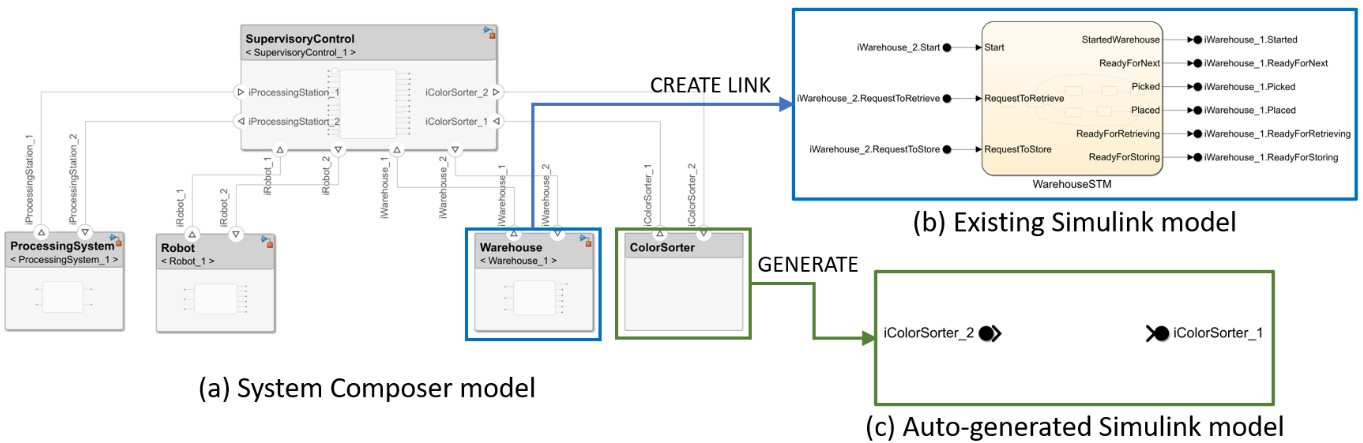
\includegraphics[width=\textwidth]{figures/03StandDerTechnik/Simulink_System_Composer.png}
  \caption{Verknüpfung einer System Composer Architektur mit einem Simulink Verhaltensmodell. (Entnommen aus \cite{chatterjee2020applications})}
  \label{fig:simulink_system_composer}
\end{figure}

Wie diese enge Integration praktisch umgesetzt wird, ist in Abbildung~\ref{fig:simulink_system_composer} zu erkennen: Eine in System Composer entworfene Architekturkomponente wird direkt mit einem detaillierten Verhaltensmodell in Simulink verknüpft. Der diesem Vorgehen zugrundeliegende Arbeitsablauf folgt dem V-Modell, bei dem das Systemverhalten phasenweise modelliert und validiert wird \cite{themathworksinc.2025system}. Um komplexe und Verhaltensweisen modellieren zu können, werden spezielle Werkzeuge innerhalb von Simulink genutzt \cite{chatterjee2020applications}:

Stateflow dient zur Modellierung der Logik von Systemen mittels Zustandsautomaten, Flussdiagrammen oder Wahrheitstafeln. Es wird insbesondere für die übergeordnete Steuerung (Supervisory Control) und dem Fehlermanagement genutzt \cite{chatterjee2020applications}. Die Fähigkeit, ereignisdiskrete Systeme zu modellieren/ analysieren, wird durch SimEvents ermöglicht. Mithilfe von Nachrichten- und Entitätenbasierten Konzepten können Leistungsmerkmale wie der Durchsatz oder die Latenz optimiert werden \cite{chatterjee2020applications}.

Wie auch bei PREEvision, unterstützt dieser gesamte Ansatz die zentralen System-Engineering Prinzipien: Abstraktion, Dekomposition und Wiederverwendung\cite{themathworksinc.2025system}.

\subsection{Eclipse Capella}
Capella ist ein nicht-kommerzielles Modellierungswerkzeug, das auf der Engineering-Methode ARCADIA\footnote{ARChitecture Analysis and Design Integrated Approach} basiert \cite{roques2016mbse}. Diese umfassende Methodik gibt einen klaren, schrittweisen Konstruktionsprozess vor, der den Anwender von der Bedarfsanalyse bis zum detaillierten Architektur-Design führt \cite{let}.

\begin{figure}
  \centering
  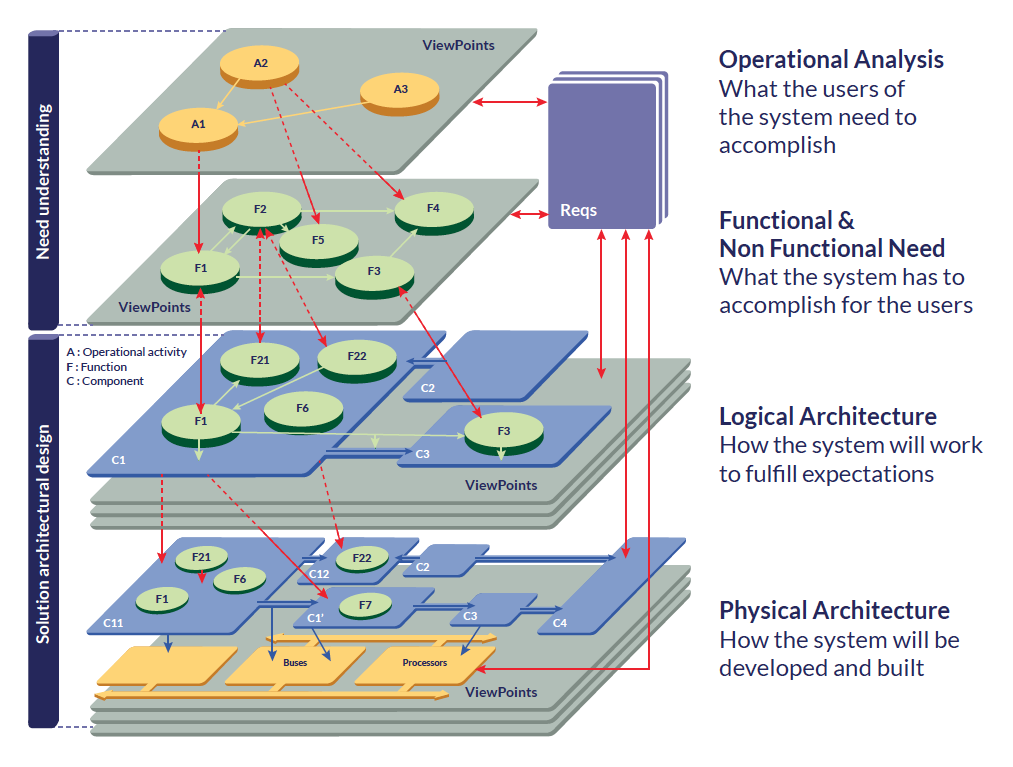
\includegraphics[width=.7\textwidth]{figures/03StandDerTechnik/phases_arcadia.png}
  \caption{Das Arcadia-Vorgehensmodell in Capella als vier übereinander gestapelte Architekturebenen (Entnommen aus \cite{let})}
  \label{fig:capella_modell}
\end{figure}

Die Abbildung~\ref{fig:capella_modell} zeigt die vier Konstruktionsphasen von Arcadia. Der Prozess beginnt mit der Betriebsanalyse, die analysiert, was die Erwartungen, Anwendungsbedingungen, Integrations-, Verifikations- und Validierungsvorraussetzungen des Endnutzer sind. Darauf aufbauend folgt die Funktionale \& Nicht-Funktionale Bedarfsanalyse, in der die Systemfunktionen und nicht-funktionalen Anforderungen abgeleitet werden.

Bei Arcadia haben Bedarfsanalyse und Modellierung, Architekturentwicklung und -validierung sowie Anforderungsanalyse die gleiche Wichtigkeit. Wobei die Anforderungen gegen eine frühe Version des Architekturmodells auf Robustheit und Machbarkeit geprüft werden.

Nachdem System, Hardware und Software modelliert wurden, wird eine logische Architektur entwickelt. Dabei wird nach einem Kompromiss zwischen Entwurfsfaktoren, (nicht-funktionalen) Bedingungen und Ansichten gesucht. Jede Ansicht beschäftigt sich mit bestimmten Aspekten wie funktionale Konsistenz, Schnittstellen, Leistung, Echtzeit, Sicherheit, Integration, Wiederverwendung, Kosten und Risiko.

Abschließend beschreibt die physische Architektur die Umsetzung auf konkrete Hardware- und Softwarekomponenten und sichert durch die Trennung der Aspekte, Schichtenarchitekturen und standardisierte Interaktionsmuster eine effiziente, sichere Entwicklung und IVVQ\footnote{Integration, Verifizierung \& Validierung, Qualifizierungsaktivitäten (Testing)} \cite{let}.

Während Arcadia die komplette linke Seite des V-Modells abdeckt, deckt das Produktlebenszyklusmanagement (PLM) die rechte Seite des Modells ab und garantiert somit eine vollständige Umsetzung des V-Modells \cite{2024arcadia}.

\section{Validierungsverfahren im Detail}

Ein zentraler Aspekt moderner Architekturwerkzeuge ist die Fähigkeit, entworfene Modelle zu validieren und deren Qualität sicherzustellen. Die in dieser Arbeit analysierten Werkzeuge verfolgen dabei unterschiedliche Ansätze und decken verschiedene Bereiche der Architekturvalidierung ab, die in Tabelle~\ref{tab:validierungsvergleich} vergleichend dargestellt werden.

\begin{table}[h!]
  \centering
  \footnotesize % Kleinere Schriftgröße für maximale Kompaktheit
  \begin{tabularx}{\textwidth}{X c c c}
    \toprule
    \textbf{Validierungsart}          & \textbf{PREEvision} & \textbf{Capella} & \textbf{Simulink} \\
    \midrule
    \multicolumn{4}{l}{\textit{Modell-Integrität \& Konsistenz}}                                   \\
    Inkonsistenz/Vollständigkeit      & \checkmark          & \checkmark       & \checkmark        \\
    Nachverfolgbarkeit                & \checkmark          & \checkmark       & \checkmark        \\
    Ebenenübergreifende Realisierung  & \checkmark          & \checkmark       &                   \\
    \midrule
    \multicolumn{4}{l}{\textit{Anforderungs- \& Design-Validierung}}                               \\
    Validierung gegen Anforderungen   & \checkmark          & \checkmark       & \checkmark        \\
    Analyse von Designalternativen    & \checkmark          & \checkmark       & \checkmark        \\
    \midrule
    \multicolumn{4}{l}{\textit{Quantitative Analysen \& Metriken}}                                 \\
    Performance-Analyse               & \checkmark          & \checkmark       & \checkmark        \\
    Netzwerk- und Ressourcen-Metriken & \checkmark          &                  &                   \\
    Statische Analyse                 &                     & \checkmark       & \checkmark        \\
    \midrule
    \multicolumn{4}{l}{\textit{Sicherheits- \& Zuverlässigkeitsanalysen}}                          \\
    Sicherheitsanalysen               & \checkmark          & \checkmark       &                   \\
    Fehlerfortpflanzungsanalyse       &                     & \checkmark       &                   \\
    \midrule
    \multicolumn{4}{l}{\textit{Verhaltensbasierte Validierung}}                                    \\
    Dynamische Simulation             &                     &                  & \checkmark        \\
    \midrule
    \multicolumn{4}{l}{\textit{Versions-Validierung}}                                              \\
    Prüfung von Modellversionen       & \checkmark          & \checkmark       & \checkmark        \\
    \bottomrule
  \end{tabularx}
  \caption{Auflistung der Architekturvalidierungen nach Werkzeug}
  \label{tab:validierungsvergleich}
\end{table}

Eine kurze Analyse der ausgewählten Werkzeuge zeigt, dass jedes von ihnen seine spezifischen Stärken in unterschiedlichen Bereichen der Architekturvalidierung besitzt. Während PREEvision bei E/E-spezifischen Metriken wie Netzwerk- und Ressourcenmetriken sowie Sicherheitsanalysen dominiert \cite{schauffele2016architectural}, liegen die Stärken von Capella in der Sicherstellung der Architekturkonsistenz über mehrere Ebenen hinweg \cite{roques2016mbse}. Als einziges Werkzeug bietet Simulink zudem die Möglichkeit zur dynamischen Validierung des Systemverhaltens mittels ausführbarer Simulation \cite{themathworksinc.2025system}.

In der Praxis ergibt sich durch diese hohe Spezialisierung eine zentrale Herausforderung: Keines der Werkzeuge deckt alle notwendigen Validierungsverfahren ab. Darüber hinaus sind diese Systeme meist geschlossene Plattformen. Die Anbindung neuer oder unternehmensspezifischer Validierungsalgorithmen, die vom Hersteller nicht vorgesehen sind, ist häufig gar nicht oder nur mit erheblichem Aufwand möglich. Es fehlt an flexiblen und offenen Schnittstellen zur Integration externer Algorithmen.

\break
Genau an dieser Stelle setzt die Bachelorarbeit an. Ziel dieser Arbeit ist es, das generische, webbasierte \textit{ArchitekturTool} um ein Framework zur automatisierten Architekturvalidierung zu erweitern. Durch die Implementierung einer offenen API-Schnittstelle soll die bestehende Lücke hinsichtlich mangelnder Flexibilität geschlossen und die einfache Anbindung beliebiger Validierungsalgorithmen ermöglicht werden.
%TODO: AUSGEWÄHLTE VALIDIERUNGSVERFAHREN
%TODO: MEIN BEITRAG

% !TEX root = ../main.tex

\chapter{Inhaltsspezifische Überschrift}
%\chapter{Very Specific Title}
\label{sect:corechapter}

% Kernstück der Arbeit (eventuell auch in mehrere Kapitel unterteilt). Hier wird konkret vorgestellt, was entwickelt wurde und wie dies von statten ging.
% This chapter (maybe split in multiple) is the main part of the thesis. It presents what was realized, how things were realized, 

As already stated before in chapter \ref{sect:chaptsect}, every chapter or section should start with some introducing words.
Due to the fact that this chapter (or potentially multiple chapters) presents the authors efforts, each section and chapter shall provide analogous to its introduction some concluding words, summarizing the findings and achievements of the specific section or chapter.


% Alles aus dem Grundlagen-Kapitel kann ohne weitere Erklärung genutzt werden. nicht zu erwarten ist, dass der leser über nicht präsentierte Zusatzinformationen zum Thema verfügt.
% The information presented before in the background chapter can be used without further explanation. However you should not assume that the reader knows further details on the topic which were not presented in this thesis.
\section{Different Citation Types}

During the writing of a thesis work, ideas and contributions provided by other people then the author have to be declared as such.
This is done using citations.
In general, there are two different types of citations.
The first type of citation is the literal citation.
It is only used if text is copied directly without modification from others.
In this case the citation is surrounded by quotes "".
For instance:
\begin{center}
Wikipedia states that \enquote{Wörtliche Zitate sollten eingesetzt werden, wenn nicht nur der Inhalt der Aussage, sondern auch deren Formulierung von Bedeutung ist} \cite{wikicite}.
\end{center}
Nonetheless, the author has to make unambiguously clear where the citation originates from.
In case of the wikipedia citation above this is done with: \cite{wikicite}.


The second citation type is the more frequent used reference using the \textbackslash cite\{\} command presented in Sect.~\ref{sect:citations}.
This citation type is used if no literal citation is used.
For instance:
\begin{center}
If not only the content of a statement is of importance but also the original wording, then literal citation using quotes has to be used \cite{wikicite}.
\end{center}
Such references have to follow directly the first statement taken from other sources.

The following example shows how this looks for bigger paragraphs.
The same colored parts refer to the same source.

\begin{flushleft}
\textcolor[rgb]{1,0,0}{Welche Theorien standardmäßig von einem Programm zur Lösung von SMT-Problemen unterstützt werden hängt vom konkret verwendeten Programm ab \cite{smtappetizer}.
Zur Vereinheitlichung der Beschreibung von Theorien, so wie der Eingabe- und Ausgabesprache für Programme die SMT-Probleme lösen wurde der SMT-LIB Standard verfasst.}
\textcolor[rgb]{0.2,0.8,0.2}{Aktuell befindet sich dieser von der SMT-LIB Initiative formulierte Standard in Version 2.0 \cite{smtlib}.}
\textcolor[rgb]{0,0.8,1}{Zu diesen Theorien gehören die Theorie der Felder (engl. \textit{arrays}), der Bit-Vektoren fester Größe, der booleschen Operatoren, der Fließkommazahlen, der Ganzzahlen, der reellen Zahlen und der Kombination von reellen und ganzen Zahlen \cite{smtlibweb}.}
\end{flushleft}

Please ensure that the visual look of the automatically generated bibliography is consistent and the printed information is complete.
For instance:
\begin{itemize}
	\item the separation of words at the end of a line should be adequate
	\item the ISBN, DOI, etc. are formatted the same way for every bibliography entry
	\item every web-sources accessing-date is stated
	\item URLs are displayed the way they are intended to (e.g. underscores in copied links are interpreted by latex as commands and not displayed unless the url is surrounded by \textbackslash url\{\} or backslashes are interpreted as escaping characters and should be replaced with \textbackslash textbackslash)
\end{itemize}
It is the responsibility of the author of a thesis to ensure that all relevant information about the used literature is readable in the printed version of the thesis.

The next section gives advice on figures used in the document and extends the citation concept accordingly.


\section{Citations and Advice on Illustrations}

Similar to textual content, pictures may originate from other publications, too.
Thus, they have to be declared as results of work from others.
In case the figure is not modified in any way this can be done by adding a correspondent citation in the figures caption.
If the figure has been redrawn or modified the reference can be given as shown below:
\begin{figure}[H]
	\centering
		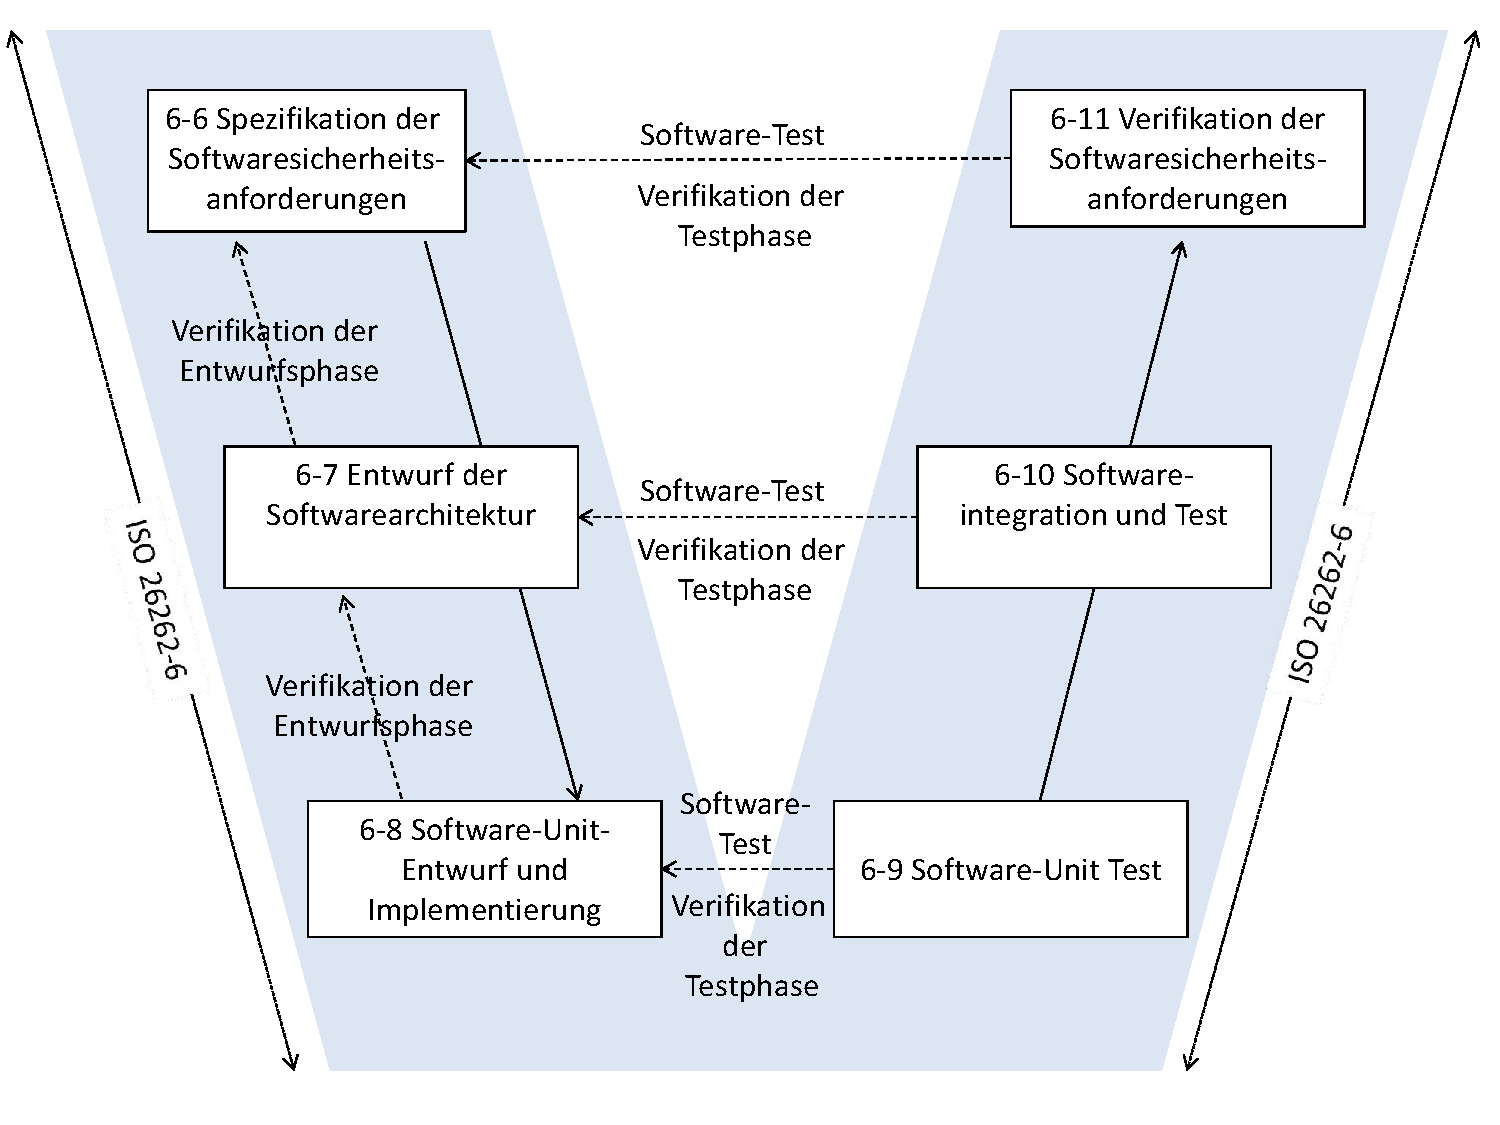
\includegraphics[width=0.80\textwidth]{figures/V-Modell.pdf}
	\caption{V-Modell correspondent to ISO 26262-6 (drawing after \cite{verificationvalidation})}
	\label{fig:vmodell}
\end{figure}

The author might even differentiate between different figure-citation-types.
Those could be:
\begin{itemize}
	\item taken from \textit{(exact copy of the figure)}
	\item partly taken from \textit{(parts of the figure are taken from the specified source, others were added by the author)}
	\item adaption/extension of
	\item redrawing of \textit{(the figure has been redrawn)}
\end{itemize}
If such descriptions or correspondent abbreviations are used the author should specify upfront the semantic and syntax at the beginning of the thesis.
The important thing here is not which words were used but that it is clear which parts are whose work.
\\\\
\textsl{\textcolor[rgb]{0.75,0.75,0.75}{It follows an example for a bad structuring of paragraphs and transition between such since the quality of figures does not relate to figure citations.}}
Also it is not recommendable to use fonts, \textcolor[rgb]{1,1,0}{colors} and other \textsl{\textit{\colorbox[rgb]{1,1,0.6}{\textcolor[rgb]{0.8,1,0.8}{styling}}}} elements (even in figures) which cannot be read easily.
\\\\
Figures should always be provided as vector graphics, e.g. *.svg or *.pdf files.
The benefit of such formats is their scalability without loss of quality.
Unfortunately, many pictures are not provided as such.
Hence, schemata etc. need often to be redrawn.
Some tools supporting the creation of vector graphics are:
\begin{itemize}
	\item inkscape (open source)
	\item powerpoint (create a slide composed of shapes and store it as *.pdf file) or word/excel\\
	(this should work with open office too)
	\item to be completed ...
\end{itemize}
Please note that importing non vector graphics, e.g. bitmaps, by the mentioned tools will not convert them into vector graphics.
Another aspect which should be addressed regarding figures in latex documents is the size of text inside figures.
Due to scale operations on figures (see \ref{fig:vmodell} where the width of the figure is set to 80 percent of the width of the region where text can be shown) the size of text labels in figures may change.
However, the size of the smallest text on a figure should never be smaller than the smallest text-size of the rest of the document.
Moreover the sizes of texts on figures should not change arbitrary between illustrations.

After this part of many theses follows an evaluation.
Some important points regarding the evaluation part are mentioned in the following chapter.
% !TEX root = ../main.tex


\chapter{Implementierung}
\label{ch:imp}

In diesem Kapitel wird die Umsetzung der in Kapitel~\ref{ch:KuD} definierten Konzepte und Designentscheidungen für das Framework im Detail beschrieben. Die Implementierung erfolgt als Erweiterung des bestehenden ArchitekturTools und nutzt dessen etablierten Technologie-Stack.

Zunächst wird die Backend-Implementierung vorgestellt, die sowohl die \gls{api} zur Verwaltung der Algorithmen als auch die Engine zur Ausführung der Validierungsläufe enthält. Danach wird die Implementierung der \gls{gui} erläutert, die die Komponenten zur Algorithmenverwaltung und zur Visualisierung der Ergebnisse beinhaltet. Abschließend wird die Implementierung des ersten Validierungsalgorithmus erläutert, dessen Durchführung im Rahmen der Evaluation als \gls{poc} für die Funktionsfähigkeit des Frameworks dient.

\section{Backend}
\label{sec:backendimp}

Das Backend bildet den serverseitigen Kern des implementierten Frameworks. Es ist dabei für die zentrale Logik verantwortlich und setzt die zuvor entworfenen Konzepte für  Verwaltung und Steuerung um. Die Implementierung basiert auf der Node.js-Laufzeitumgebung in Verbindung mit dem Express.js-Framework und dem Prisma ORM. Die folgenden Unterabschnitte erläutern im Detail, wie sowohl zuvor konzipierte \gls{api} zur Algorithmenverwaltung als auch die Validierungsengine umgesetzt wurden.

\subsection{Umsetzung der API}
\label{subsec:api}

Um dem Frontend die Interaktion und Verwaltung der Validierungsalgorithmen zu ermöglichen, wurde serverseitig eine \gls{rest}-\gls{api} implementiert und, die Endpunkte für alle erforderlichen CRUD-Operationen bereitstellt. Die neu implementierten Endpunkte integrieren sich in die bestehende Routing-Struktur des ArchitekturTools und sind unter dem Präfix \texttt{/api/v2/} erreichbar.

\subsubsection*{CREATE - \texttt{POST /api/v2/algorithm}}

Zum Anbinden neuer Validierungsalgorithmen dient der \texttt{POST}-Endpunkt. Zunächst wird ein eingehender Request von der \textit{Multer}\footnote{https://www.npmjs.com/package/multer}-Middleware verarbeitet, die die hochgeladene Datei aus der \texttt{multipart/form-data}-Request extrahiert und in dem vordefinierten Verzeichnis (\texttt{/uploads/algorithm}) serverseitig speichert. Die Eindeutigkeit der Algorithmen wird gewährleistet, in dem vor dem Speichern mit der von Prisma zur Verfügung gestellten Methode \texttt{prisma\_db.algorithm.findFirst()} geprüft wird, ob ein Algorithmus mit dem übergebenen Namen bereits in der \texttt{algorithm}-Datenbanktabelle existiert. Falls dies der Fall ist, wird der Request mit dem Statuscode 409 Conflict abgelehnt. Andernfalls werden die Metadaten zusammen mit dem Dateipfad durch \texttt{prisma\_db.algorithm.create()} in der Datenbanktabelle abgelegt und der neu erstellte Datensatz mit dem Created-Statuscode als \textit{Response} zurückgegeben.

\subsubsection*{READ - \texttt{GET /api/v2/algorithms}}

Um alle verfügbaren Algorithmen im Frontend darzustellen, stellt der \texttt{GET}-Endpunkt eine Liste aller Einträge innerhalb der \texttt{algorithm}-Tabelle bereit. Dies wird durch den Aufruf der Prisma-Methode \texttt{prisma\_db.algorithm.findMany()} umgesetzt, die alle Datensätze abruft und als JSON-Array an das Frontend übermittelt.

\subsubsection*{UPDATE - \texttt{PATCH /api/v2/algorithm/:id}}

Zur Aktualisierung eines bestehenden Validierungsalgorithmus wird der \texttt{PATCH}-Endpunkt genutzt. Anhand der in der \textit{URL}\footnote{Uniform Resource Locator} übergebenen \texttt{:id}, wird der dazugehörige Datensatz mittels \texttt{prisma\_db.algorithm.findunique()} aus der \texttt{algorithm}-Tabelle abgerufen. Wird im Rahmen des Requests eine neue Datei hochgeladen, wird die alte, dazugehörige Datei zunächst mit der Node.js-Funktion \texttt{fs.unlinkSync} vom Server gelöscht, um Dateien ohne Zugehörigkeit zu vermeiden. Anschließend werden die aktualisierten Metadaten sowie der neue Dateipfad mithilfe von \texttt{prisma\_db.\\ algorithm.update()} in der \texttt{algorithm}-Tabelle gespeichert.

\subsubsection*{DELETE - \texttt{DELETE /api/v2/algorithm/:id}}

Der \texttt{DELETE}-Endpunkt dient dem vollständigen Löschen eines Algorithmus. Um die Konsistenz des Systems sicherzustellen, folgt die Implementierung dieses Endpunkts einem zweistufigen Prozess: Zu Beginn wird der Datensatz anhand der übergebenen \texttt{:id} aus der Datenbank gelesen, um den Pfad zur entsprechenden Datei zu ermitteln. Diese Datei wird im Anschluss über \texttt{fs.promises.unlink} vom Dateisystem des Servers entfernt. Danach wird im zweiten Schritt der Datenbankeintrag selbst über \texttt{prisma\_db.algorithm.delete()} aus der Datenbanktabelle gelöscht. Mit diesem Ablauf wird sichergestellt, dass, wie beim \texttt{UPDATE}-Endpunkt, keine verwaisten Dateien auf dem Server zurückbleiben

\subsection{Integrierung der Validierungs-Engine}
\label{subsec:engine}

Die Durchführung der Validierungsläufe bildet die Schlüsselfunktionalität des Backends. Sie ist dafür zuständig die Daten aufzubereiten, die kontrollierte Ausführung eines isolierten Python-Prozesses sowie die Verarbeitung und Abspeicherung der Ergebnisse. Dieser Prozess wird durch einen dedizierten \gls{api}-Endpunkt gestartet.

Der komplette Ablauf eines Validierungslaufs, von der Aufbereitung der Daten über die Ausführung des isolierten Python-Prozess, bis hin zur Speicherung des Ergebnisses, ist ein aufeinander abgestimmter Prozess. Abbildung~\ref{fig:seqvalid} verdeutlicht das Zusammenspiel der beteiligten Komponenten.

\begin{figure}[h!]
  \centering
  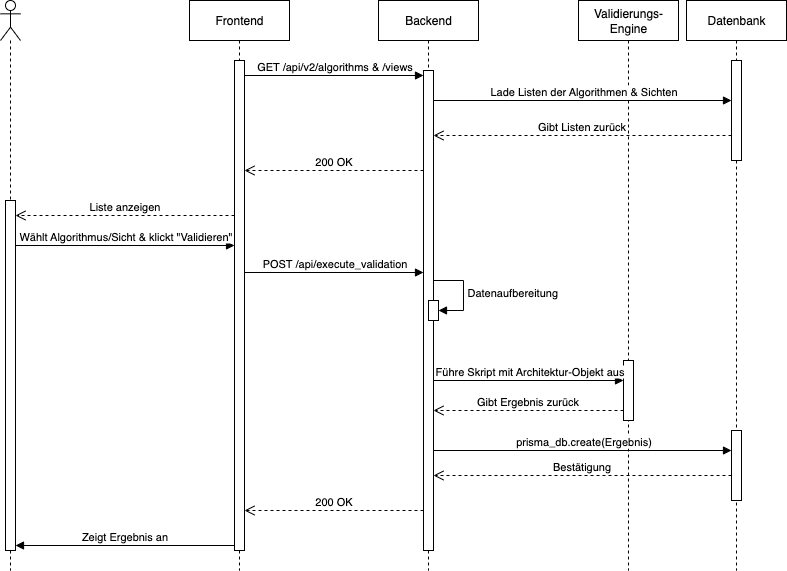
\includegraphics[width=\textwidth]{figures/05Implementierung/Sequenz_valid.drawio.png}
  \caption{Verlauf einer Architekturvalidierung im Framework}
  \label{fig:seqvalid}
\end{figure}

\subsubsection*{Datenaufbereitung und Export}

Nachdem der Request mit den IDs für den Algorithmus und der Architektursicht validiert wurde, stellt die Engine die erforderlichen Komponentendaten bereit. Hierfür wird auf eine angepasste Version des bestehenden \textit{JSON-Exporter} des ArchitekturTool zurückgegriffen.

Die Engine prüft zunächst, ob die Komponenten der angeforderten Sicht bereits als Datei im JSON-Format auf dem Server liegen. Falls nicht, wird der Exportprozess automatisch gestartet, der die Komponentendaten aus der Datenbank extrahiert und in einem sichten-spezifischen Ordner abgelegt. Anschließend werden diese JSON-Dateien eingelesen und zu einem einzigen Architektur-Objekt zusammengefügt, das als Eingabe für den Validierungsalgorithmus dient.

\subsubsection*{Durchführung des Python-Prozess}

Die eigentliche Validierung wird in einem isolierten Python-Prozess durchgeführt, um die Stabilität des Servers zugewährleisten. Hierfür wird die \texttt{spawn}-Funktion aus dem \texttt{child\_process}-Modul von Node.js genutzt. Diese startet das Python-Skript, das zum ausgewählten Algorithmus gehört. Das zuvor erstellte Architektur-Objekt wird als JSON-String in den Standard-Input des Python-Prozesses geschrieben. Eventuelle Probleme beim Starten des Prozesses werden vom Error-Listener abgefangen.

\subsubsection*{Ergebnisverarbeitung}

Gegen Ende der Durchführung nimmt das Backend die Standardausgabe und die Fehlerausgabe des Python-Skripts entgegen. Wenn ein Fehler auftritt, wird der Validierungslauf als fehlgeschlagen gewertet und ein entsprechender Eintrag mit der entsprechenden Fehlermeldung in der \texttt{result}-Tabelle der Datenbank gespeichert. Anhand der Definierung der Struktur des Objekts wird der Ergebnistyp dynamisch als \texttt{TEXT} oder \texttt{METRIC} bestimmt. Schließlich wird das Ergebnis gemeinsam mit den Metadaten wie der Ausführungsdauer und dem Erfolgsstatus mithilfe von Prisma auch in der \texttt{result}-Tabelle abgespeichert und zur Visualisierung an das Frontend gesendet.

\section{Frontend}
\label{sec:frontendimp}

Die \gls{gui} wurde mit React entwickelt und folgt einer modularen, komponentenbasierten Architektur, was eine klare Trennung der Zuständigkeiten ermöglicht. Ein übergeordneter \texttt{ValidationContainer} verwaltet den gesamten Anwendungszustand wie Ladeindikatoren, Fehler, Ergebnisse und Validierungsverlauf. Dieser Zustandshalter gibt Daten sowie Callback-Funktion über Props an  die untergeordneteten Komponennten weiter. Zur Speicherung des Verlaufs über die Browsersitzung hinweg nutzt der Zustandshalter den \texttt{localStorage} des Browser.

\subsection{Algorithmenverwaltungs-Komponenten}
\label{subsec:verwaltung}

Die Verwaltung der Algorithmen ist die zentrale Interaktionsstelle für den Nutzer. Diese besteht aus einer Hauptkomponente zur Steuerung und einem modalen Fenster zum Erstellen, Bearbeiten und Löschen der Algorithmen.

\subsubsection*{Hauptkomponente}

Die zentrale Steuereinheit ruft bei ihrer Initialisierung mithilfe der Lebenszyklus-Methode \texttt{componentDidMount} über \textit{axios}\footnote{https://axios-http.com/docs/intro} asynchron jeweils die \texttt{GET}-Request die Algorithmen und die Architektursichten auf. Die erhaltenen Daten werden lokal im Zustand der Komponente gespeichert und dazu genutzt, die beiden Auswahllisten zu füllen. Die \texttt{onChange}-Handler dieser Listen aktualisieren den Zustand, sobald ein Algorithmus bzw. eine Sicht ausgewählt wurde.

Ein Klick auf den dedizierten \glqq Validieren\grqq{}-Button startet den in Abschnitt~\ref{subsec:engine} beschriebenen Validierungslauf. Dabei wird eine \texttt{POST}-Request mit der \texttt{algorithmId} und \texttt{viewId} als Parameter an den entsprechenden Endpunkt gesendet. Mittels einer Callback-Funktion wird der Fortschritt und das Ergebnis dieses Durchlaufs an die übergeordnete Container-Komponente gesendet.

\subsubsection*{Modalfenster}

Für das Hochladen, Bearbeiten und Entfernen der Algorithmen wird die Komponente \texttt{AlgorithmModal} genutzt die ein seperates Fenster öffnet. Dieses modale Fenster unterscheidet zwischen einem Hochladungs- und einem Bearbeitungsmodus, abhängig davon, ob eine \texttt{selectedAlgorithm}-Prop übergeben wird. Im Bearbeitungsmodus wird das Formular bereits mit den jeweiligen Daten vorbefüllt. Dem Nutzer wird es mithilfe des integrierten \textit{Monaco-Editors}\footnote{https://microsoft.github.io/monaco-editor/} ermöglicht, Python-Code direkt im Browser zu schreiben, einzufügen und zu bearbeiten. Um dem Nutzer dabei den Einstieg zu erleichtern und die Konsistenz der Algorithmen zu gewährleisten, wird ein Code-Gerüst als Vorlage bereitgestellt, wie in Abbildung~\ref{fig:codeskeleton} dargestellt wird.

Die Ziele beim Anbinden neuer Algorithmen. sind das Vereinfachen und das Standardisieren:

\begin{itemize}
  \item \textbf{Verringern von Boilerplate-Code:} Das Gerüst enthält eine \texttt{main}-Funktion, die die gesamte Interaktion mit der Engine zusammenfasst. Sie übernimmt das Einlesen der Architektur über den Input, die Fehlerbehandlung bei ungültigem JSON sowie das Schreiben des Ergebnis-Objekts auf den Output. Nutzer müssen sich somit nicht mit dem wiederkehrenden Teil des Codes befassen.
  \item \textbf{Klar definierter Bereich:} Durch die vorgegebene Struktur, ist die einzige Aufgabe des Nutzers, die Funktion \texttt{run\_validation\_algorithm} mit der eigentlich Validierung zu füllen. Somit wird sichergestellt, dass der Fokus nur auf das Prüfen der Logik liegt.
  \item \textbf{Bereitstellung gängiger Bibliotheken:} Wie in Abbildung~\ref{fig:codeskeleton} zu sehen ist, importiert das Gerüst bereits einige in der Architekturvalidierung etablierten Bibliotheken, darunter \texttt{pandas}, \texttt{numpy}, \texttt{matplotlib} und \texttt{cantools}. Damit wird eine einheitliche und leistungsstarke Entwicklungsumgebung geschaffen. Zudem kann man manuell weitere Bibliotheken hinzufügen, indem man diese in der \texttt{py-libraries.txt} hinein schreibt.
  \item \textbf{Definierte Ergebnisstruktur:} Das Gerüst gibt durch die Dokumentation eine klare Struktur für das Ergebnis-Dictionary vor. Der Nutzer legt durch die Wahl der Schlüsselbegriffe im zurückgegebenen Dictionary fest, wie das Ergebnis zu interpretieren ist. Diese Struktur ist entscheidend, da sie vom Backend ausgelesen wird, um den Typen des Ergebnisses (\texttt{TEXT} oder \texttt{METRIC}). zu bestimmen. Damit wird es dem Frontend ermöglicht, ohne weitere Konfiguration die passende Visualisierungskomponente zu wählen.
\end{itemize}

Beim Speichern wird der Code aus dem Editor in ein \texttt{Blob}- und anschließend in eine \texttt{File}-Objekt umgewandelt. Der code wird zusammen mit den Metadaten aus dem Formular über eine \texttt{POST}- oder \texttt{PATCH}-Request an das Backend gesendet. Zusätzlich ist eine Löschfunktion implementiert, die mit einer \texttt{DELETE}-Request die entsprechenden Einträge entfernt.

Der vollständige Prozess des Anbinden eines Validierungsalgorithmus, von der Eingabe des Nutzers im Modalfenster, bis zum finalen speichern, wird in Abbildung~\ref{fig:anbindung} als Sequenzdiagramm veranschaulicht.

\begin{figure}[h!]
  \centering
  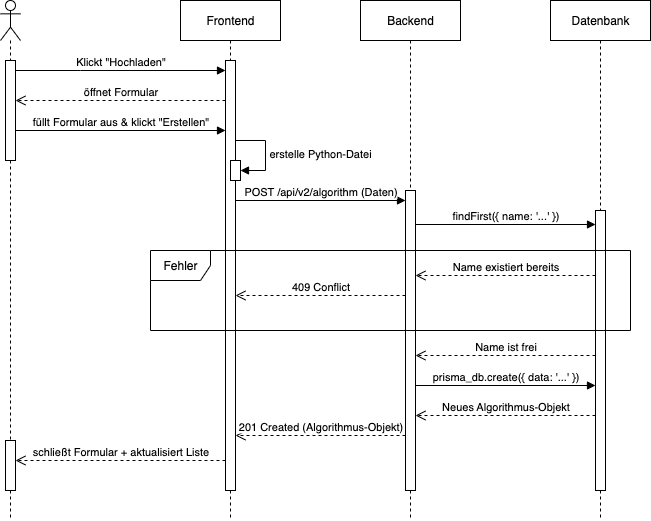
\includegraphics[width=\textwidth]{figures/05Implementierung/Sequenz_Algo_erstellen.drawio.png}
  \caption{Anbindungsprozess innerhalb des Validierungs-Frameworks}
  \label{fig:anbindung}
\end{figure}

Wie in der Abbildung dargestellt, wird vom Frontend aus ein \texttt{POST}-Request an das Backend gesendet. Dabei ist ein wichtiger Aspekt die anschließende Prüfung auf einen Namenskonflikt, bevor der neue Datensatz in der Datenbank abgespeichert wird.

\subsection{Visualisierung der Ergebnisse}
\label{subsec:visual}
Die Darstellung der Ergebnisse ist ebenso wie die Algorithmenverwaltung, modular aufgebaut, um verschiedene Ergebnistypen und eine Ergebnishistorie abzubilden. Sie unterteilt sich in die dynamische Darstellung des aktuellen Ergebnisses, mit der zugrundeliegenden Graphenvisualisierung und dem Verlauf der Validierungsdurchläufe.

Mithilfe dieser Komponente wird das Validierungsergebnis der aktuellen Ausführung visualisiert. Ihr gerenderter Inhalt wird durch die vom Container übergebenen Props gesteuert.

Das Kernstück dieser Komponente ist das dynamische Rendern der Ergebnisse, das auf den \texttt{resultType}-Prop basiert. Hier wird mittels \texttt{switch}-Anweisung, je nach Ergebnistyp, die passende Visualisierung ausgewählt:

\begin{itemize}
  \item \textbf{Textuelle Ausgabe(\texttt{TEXT}):} Standardmäßig werden die Ergebnisse als JSON in einem \texttt{<pre>}-Element dargestellt. Wie dieser formatiert sein soll bestimmt der Nutzer in seinem Python-Code.
  \item \textbf{Metrische Ausgabe(\texttt{METRIC}):} Bei metrischen Ergebnisdaten wird die Komponente Diagramm-Visualisierung instanziiert. Ihr werden die Messwerte und Grenzwerte als Props übergeben, woraufhin die Komponente die Darstellung als Linien-, Balken- oder Flächendiagramm übernimmt.
\end{itemize}

Der Ansatz des dynamischen Rendern stellt sicher, dass das Frontend flexibel auf unterschiedliche Ausgabeformate der Algorithmen reagieren kann, ohne dass Änderungen an der Komponente vorgenommen werden müssen.

\subsubsection*{Diagramm-Visualisierung}

Die Visualisierung der metrischen Daten baut auf der populären Bibliothek \textit{Recharts}\footnote{https://recharts.org/en-US} auf, die mit den gelieferten Daten in eine interaktive und auswertbare grafische Form überführt wird (Siehe Abbildung~\ref{fig:metricvis}).

Der Ablauf innerhalb dieser Komponente ist wie folgt:

\begin{enumerate}
  \item \textbf{Normalisierung der Daten:} Zunächst werden die eingehenden Daten durch eine Funktion aufbereitet und normalisiert. Diese Funktion extrahiert aus den Datenpunkten eine einheitliche Bezeichnung für die X-Achse, die entweder aus einem \texttt{timestamp} oder \texttt{name} Feld entnommen wird. Außerdem stellt sie sicher, dass die restlichen numerischen Werte korrekt als verwertbare Datenserie für das Diagramm zur Verfügung stehen.
  \item \textbf{Dynamische Diagramm-Auswahl:} Basierend auf dem \texttt{chartType}-Prop, die vom Validierungsalgorithmus mit dem Ergebnis-Dictionary mitgegeben wird, wählt die Komponente dynamisch die passende Visualisierung aus Recharts aus (\texttt{LineChart, BarChart} oder \texttt{AreaChart}). Dies ermöglicht dem Ersteller des Algorithmus, die am besten geeignete Darstellungsform für die Metrik vorzugeben.
  \item \textbf{Visualisierung von Grenzwerten:} Ein wichtiges Feature ist es Grenzwerte visuell darzustellen. Wird ein \texttt{threshold} übergeben, rendert die Komponente eine horizontale, gestrichelte Linie in das Diagramm. Dies macht es sofort ersichtlich, ob die Messwerte innerhalb des erwarteten Bereichs liegen. Zudem wurde eine Funktion zur Prüfung jedes einzelnen Datenpunkt eines Liniendiagramms implementiert, das man in Abbildung~\ref{fig:Liniendiagramm} gut erkennen kann. Wird der Wert des definierten Grenzwerts überschritten, wird der zugehörige Punkt innerhalb des Diagramms farblich markiert.
\end{enumerate}

\begin{figure}[h!]
  \centering
  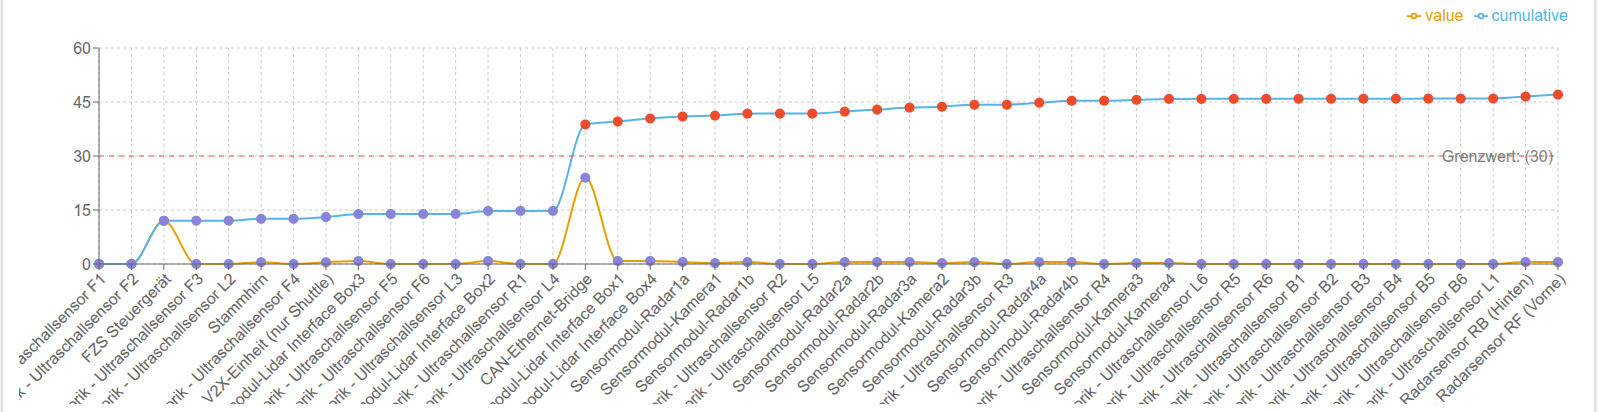
\includegraphics[width=\textwidth]{figures/06Evaluation/Line.png}
  \caption{Eine Beispielvisualisierung des Liniendiagramms samt Grenzwert visualisiert}
  \label{fig:Liniendiagramm}
\end{figure}

Des Weiteren werden UI-Elemente, wie eine Legende, Tooltips beim überfahren mit der Maus sowie beschriftete X- und Y-Achsen, gerendert um eine hohe Benutzerfreundlichkeit und eine einfache Interpretation zu gewährleisten.

\subsubsection*{Ergebnishistorie}

Um die Verfolgbarkeit der Validierungsergebenisse zu gewährleisten, wird die Komponente für die Darstellung der letzten Zehn Validierungsläufe implementiert. Hierzu wird die \texttt{history}-Prop vom übergeordneten Container empfangen, der diesen Zustand über den \texttt{localStorage}-Service des Webbrowsers auch nach einem Neuladen der Seiter erhält.

Die Ergebnisse werden hierbei in Form einer aufklappbaren Liste präsentiert, um die Benutzeroberfläche übersichtlich zu halten. Listeneinträge zeigen zunächst die wichtigsten Eckdaten bzgl. des Validierungslauf: Name des Algorithmus, die gewählte Architektursicht und dem Zeitstempel der Durchführung. Mit einem Klick auf den jeweiligen Eintrag öffnet sich dieser und visualisiert die vergangenen Ergebnisse mit derselben Darstellung wie bei der Visualisierung der aktuellen Ergebnisse. Dieser Ansatz stellt eine konsistente Nutzererfahrung sicher.
\section{Validierungsalgorithmus}
\label{sec:validimp}

Als \gls{poc} für das entwickelte Framework wird ein erster Validierungsalgorithmus implementiert. Bei dem zu realisierenden Algorithmus handelt es sich um einen Traceability-Check. Überprüfungen dieser Art sind während der Systementwicklungsphase von großer Wichtigkeit, da sie die Nachverfolgbarkeit zwischen Anforderungen und deren Umsetzung sicherstellen. Somit lassen sich Anforderungen ohne Umsetzungen sowie Garantien ohne Anforderungen aufdecken. Dabei handelt es sich um einen wichtigen Schritt, um die Vollständigkeit und Korrektheit einer Architektur zu beurteilen. Der Algorithmus wird in das Codegerüst, das in Abschnitt~\ref{subsec:verwaltung} beschrieben wurde, integriert.

Der Algorithmus wird wie folgt implementiert:
\begin{enumerate}
  \item Zunächst werden alle Komponenten des Architektur-Objekts vom Algorithmus durchlaufen. Dabei werden alle Anforderungen und Garantien in zwei verschiedenen Dictionaries gespeichert. Dies ermöglicht später einen effizienten Zugriff und einfache Nachverfolgung der Verbindungen zwischen den beiden.
  \item Danach werden die gesammelten Daten untersucht. Es werden vier Listen erstellt, in die jeweils Anforderungen und Garantien wie folgt einsortiert werden:
        \begin{itemize}
          \item Anforderungen mit zugeordneten Garantien
          \item Anforderungen ohne zugeordnete Garantien
          \item Garantien mit zugeordneten Anforderungen
          \item Garantien ohne zugeordnete Anforderungen
        \end{itemize}
  \item Abschließend wird mithilfe dieser vier Listen ein Report erstellt, die lesbar und einfach zu verstehen sein soll. Für jeden Abschnitt werden die entsprechenden Elemente aufgelistet und formartiert, wodurch der Nutzer auf einen Blick erkennen kann, welche Anforderungen noch nicht umgesetzt wurden oder welche Garantien noch keine Anforderung erfüllen.
\end{enumerate}

Im folgenden Kapitel dient dieser Algorithmus als konkreter Anwendungsfall zur Evaluation des Frameworks. Durch seine Ausführung wird die Funktionsfähigkeits der Erweiterungen nachgewiesen.

% !TEX root = ../main.tex

\chapter{Evaluation}
\label{ch:evaluation}

Dieses Kapitel dient der Evaluierung, der im Rahmen dieser Arbeit konzipierten und implementierten Erweiterung für das webbasierte ArchitekturTool. Das Hauptziel dieser Evaluation ist es nachzuweisen, dass das entwickelte Framework zur automatisierten Architekturvalidierung die zuvor definierten Anforderungen erfüllt und einen funktionalen Prozess bereitstellt.

Folgende Aspekte werden systematisch überprüft:
\begin{itemize}
  \item Die Funktionalität und Bedienbarkeit der \gls{gui} zur Initiierung der Validierungsalgorithmen.
  \item Die korrekte und verständliche Aufbereitung der Ergebnisse in der zugehörigen Komponente.
  \item Die funktionale Korrektheit der entwickelten \gls{api} als Schnittstelle zwischen Frontend und Backend.
\end{itemize}

Diese Kriterien werden anhand eines \gls{poc} überprüft. Dabei wird der in Abschnitt~\ref{sec:validimp} implementierte Validierungsalgorithmus verwendet, um das Zusammenspiel der neu entwickelten Komponenten zu demonstrieren.

Dazu wird im Folgenden zunächst   das Ergebnis der Durchführung präsentiert und im Anschluss unter Berücksichtigung der Anforderung diskutiert und bewertet.

\section{Testszenario}
\label{sec:testszenario}

In diesem Abschnitt wird die Praxisanwendung des implementierten Frameworks anhand des Traceability-Check-Algorithmus demonstriert. Der Prozess startet beim Anbinden des Algorithmus in das ArchitekturTool bis hin zur Darstellung des Validierungsergebnisses.

\subsection{Anbindung des Validierungsalgorithmus}
Eine der zentralen Funktionen des Frameworks ist die Möglichkeit, neue Validierungsalgorithmen dynamisch anzubinden. Dies erfolgt über das \glqq Algorithmus hochladen\grqq{}-Formular, in dem Metadaten wie Name, Beschreibung und der auszuführende Python-Code hinterlegt werden, das in Abbildung~\ref{fig:formularclean} zu sehen ist.

\begin{figure}[h!]
  \centering
  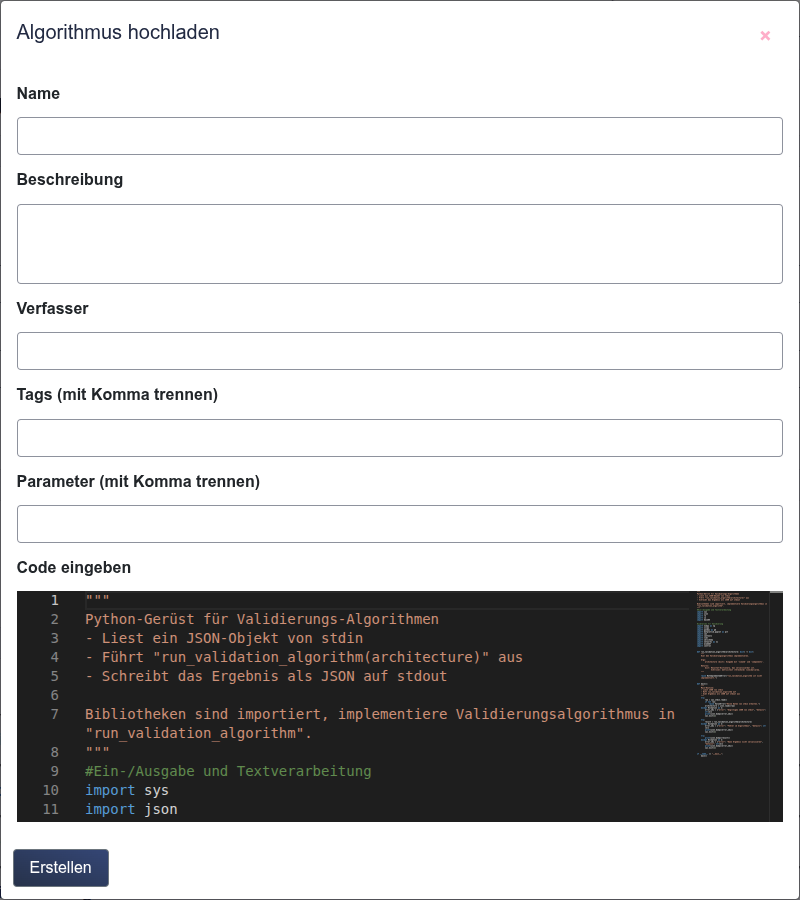
\includegraphics[width=.5\textwidth]{figures/06Evaluation/Bildschirmfoto vom 2025-08-01 11-36-46.png}
  \caption{Das Formular zum Erstellen und Hochladen des Validierungsalgorithmus}
  \label{fig:formularclean}
\end{figure}

Für diese Evaluation wird der bereits vorgestellte Traceability-Check-Algorithmus verwendet. Abbildung~\ref{fig:formularfilled} zeigt den Bearbeitungsmodus der Algorithmenverwaltung mit den im ArchitekturTool hinterlegten Details dieses Algorithmus, einschließlich Beschreibung und implementierten Codes. In diesem Modus können die angelegten Daten aktualisiert oder der Algorithmus vollständig entfernt werden.

\begin{figure}[htp!]
  \centering
  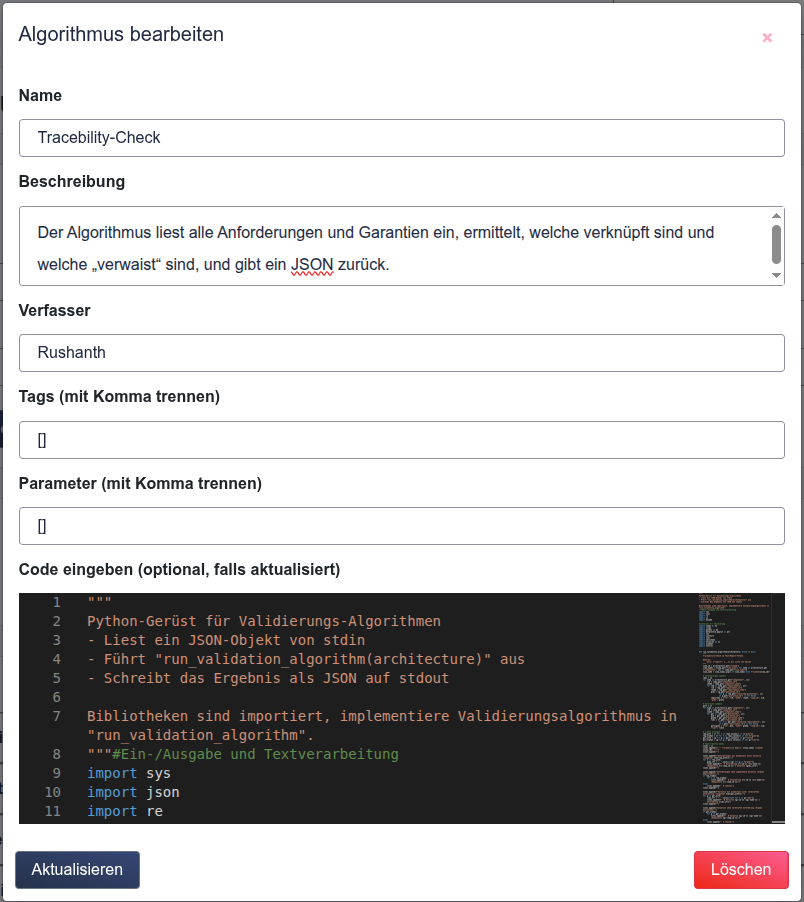
\includegraphics[width=.5\textwidth]{figures/06Evaluation/Bildschirmfoto vom 2025-08-01 11-58-21.png}
  \caption{Detailansicht des für die Evaluation genutzten Algorithmus}
  \label{fig:formularfilled}
\end{figure}

\subsection{Ausführung der Validierung und Ergebnisdarstellung}

Die Ausführung der Validierung findet in der Hauptansicht des Frameworks statt. Dafür wählt der Nutzer den gewünschten Validierungsalgorithmus, der in diesem Anwendungsbeipsiel der Traceability-Check ist, und die zu prüfende Architektursicht aus, wie in Abbildung~\ref{fig:valstart} zu sehen ist.

\begin{figure}[htp!]
  \centering
  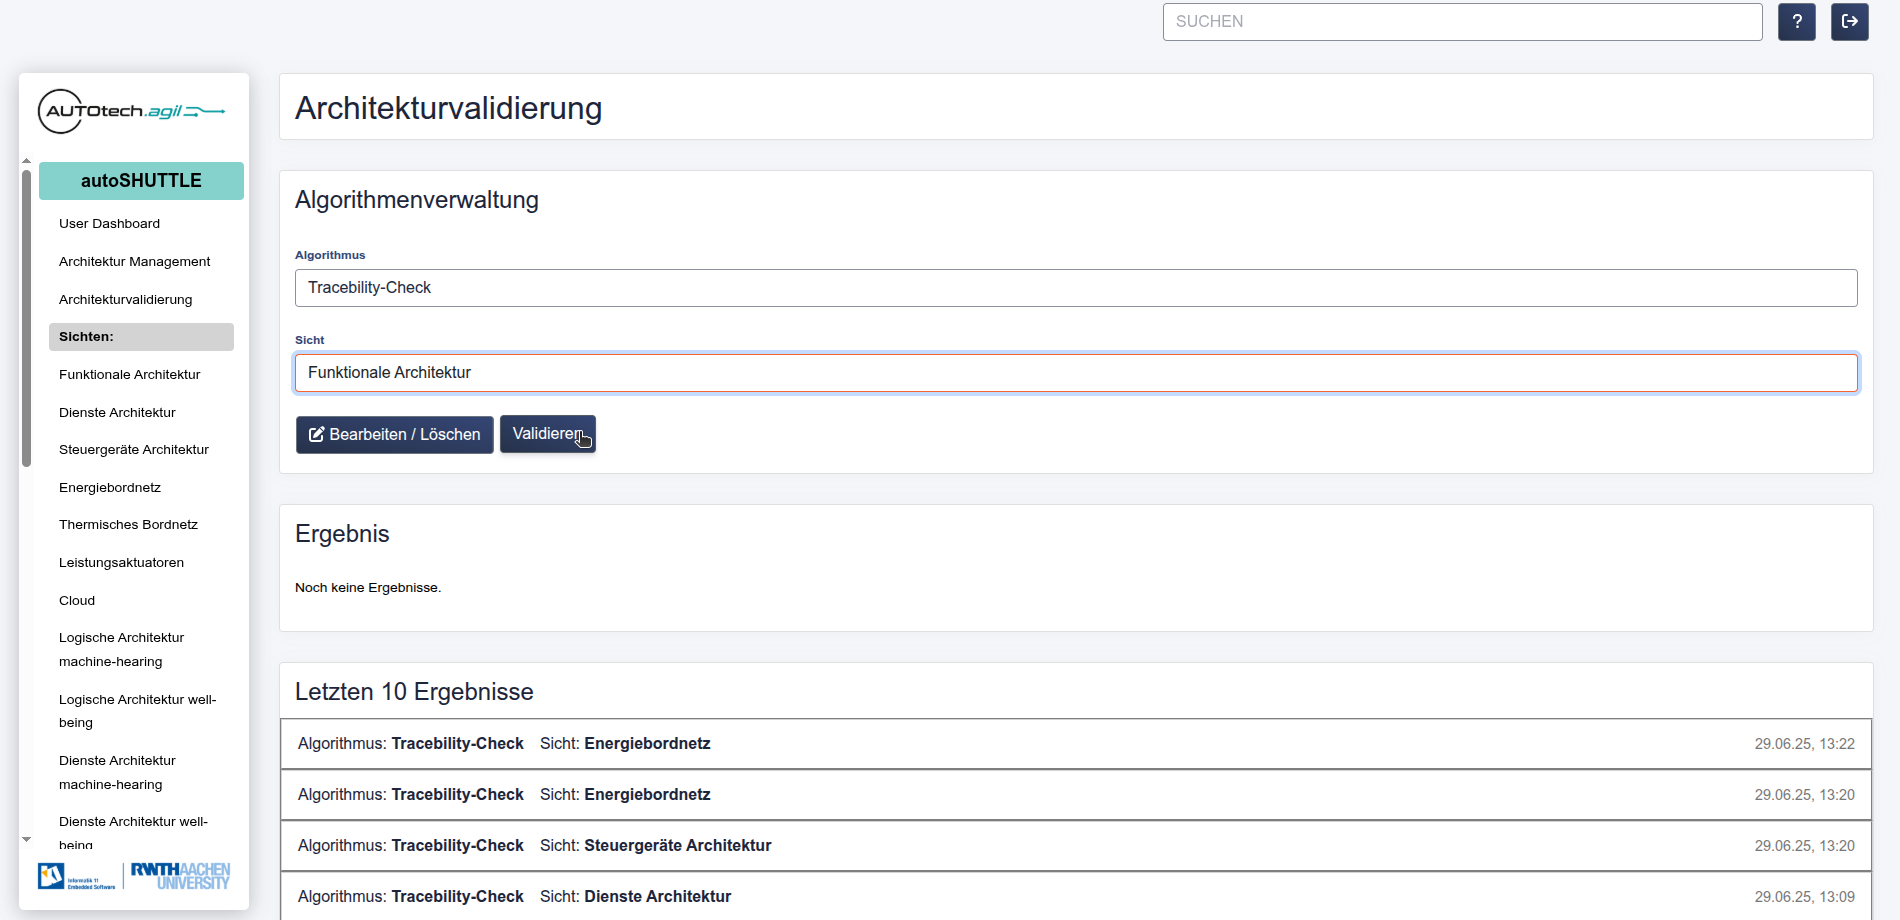
\includegraphics[width=\textwidth]{figures/06Evaluation/Bildschirmfoto vom 2025-06-30 09-16-40.png}
  \caption{Auswahl des Algorithmus und der zu validierenden Architektursicht.}
  \label{fig:valstart}
\end{figure}

Durch einen Klick auf den \glqq Validieren\grqq{}-Button wird der Prozess gestartet: Das Frontend sendet den Request über die \gls{api} an das Backend, der Algorithmus wird ausgeführt und das Ergebnis zurückgesendet.

Bei diesem Szenario wird eine Architektur verwendet, die Lücken in der Rückverfolgbarkeit enthält: Anforderungen, denen keine Garantien zugeordnet sind. Daher wird erwartet, dass der Algorithmus genau diese Anforderungen identifiziert und im Ergebnis aufzeigt.

Das Ergebnis der Ausführung ist in Abbildung~\ref{fig:valresult}, bzw. in Abbildung~\ref{fig:fullresult} ausführlich, dargestellt. Die Ausgabe entspricht den Erwartungen: Der Bericht listet die Anforderungen ohne zugehörigen Garantien auf und belegt damit, dass das Framework wie gewünscht funktioniert und Lücken in der spezifizierten Architektur aufzeigen kann.

\begin{figure}[htp!]
  \centering
  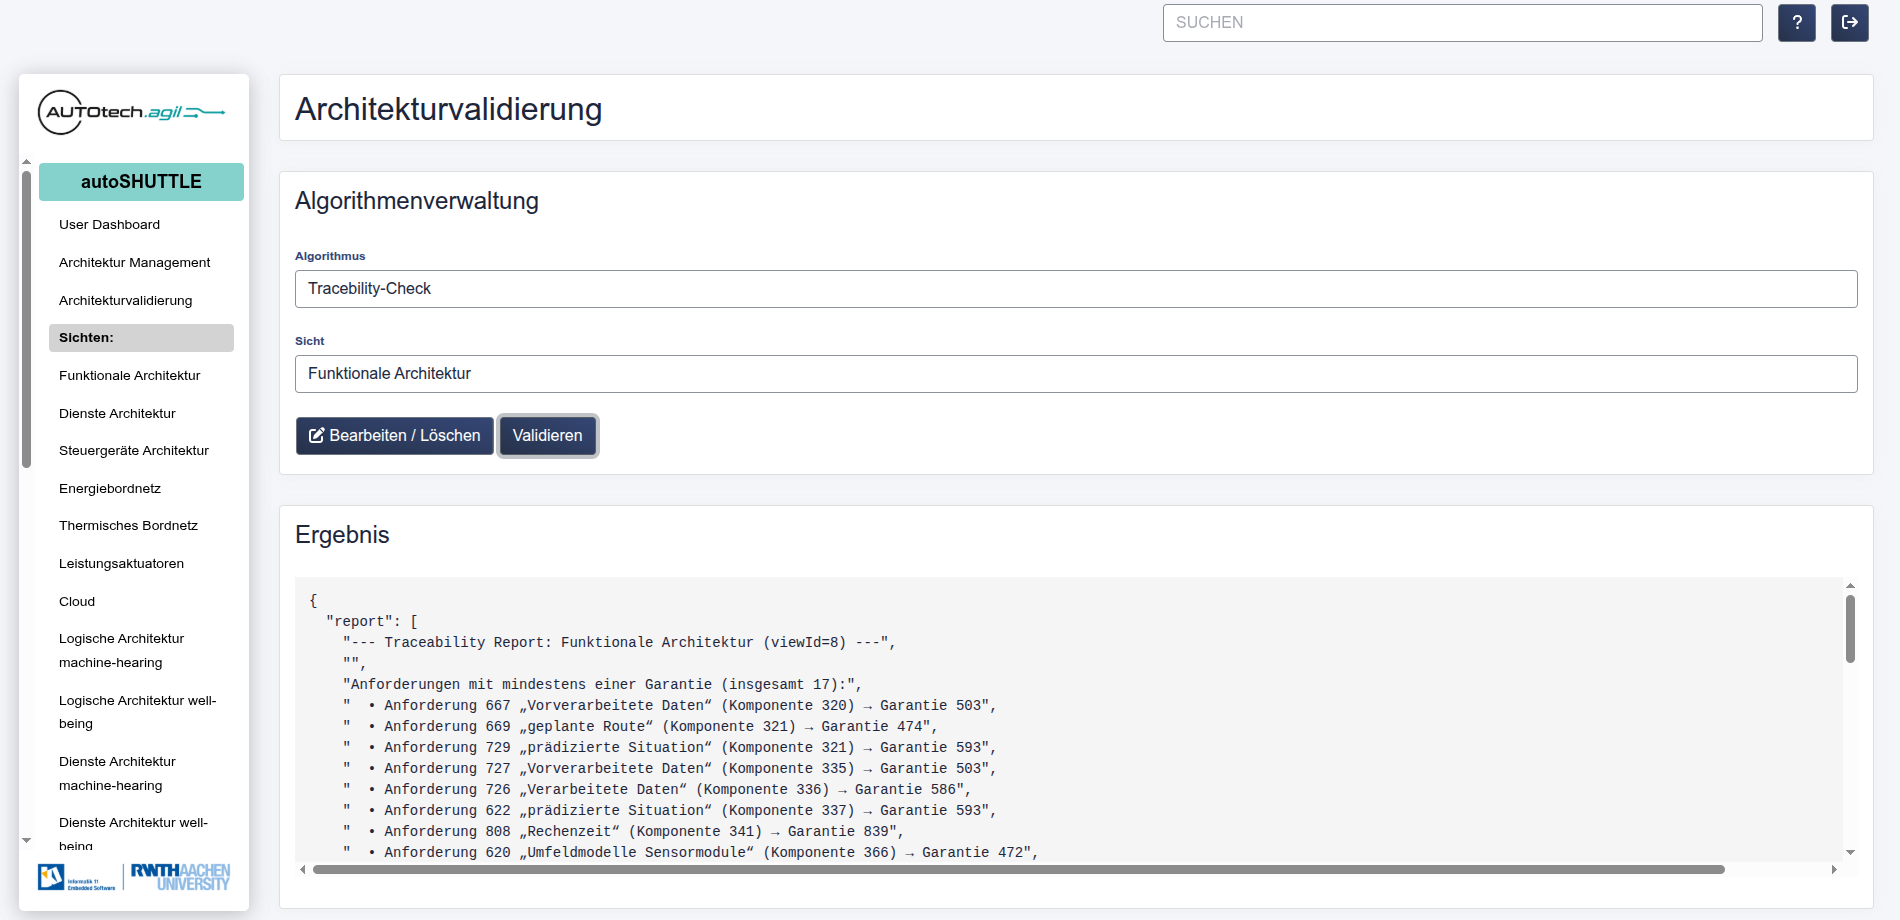
\includegraphics[width=\textwidth]{figures/06Evaluation/Bildschirmfoto vom 2025-06-30 09-17-02.png}
  \caption{Darstellung des Reports mit den korrekt identifizierten Anforderungen ohne Garantien.}
  \label{fig:valresult}
\end{figure}

Ergänzend zur Visualisierung der aktuellen Validierungsdurchläufe bietet das Framework eine weitere Komponente, in der die Ergebnisse der letzten zehn Validierungsläufe eingesehen werden können. Diese Funktionalität war nicht Teil der ursprünglichen Anforderungen an das Framework, wird hier jedoch zur Vollständigkeit erwähnt (siehe Anhang~\ref{fig:historie})

\section{Bewertung der Ergebnisse}
\label{sec:analyse}

Aufbauend auf dem Nachweis aus dem vorherigen Abschnitt werden die Ergebnisse nun bewertet und eingeordnet. Es wurde gezeigt, dass das Framework den Traceability-Check-Algorithmus ausführen und dessen Ergebnisse korrekt darstellen kann. Der Fokus der folgenden Bewertung liegt darauf, diese gezeigte Funktionalität systematisch mit den initialen Anforderungen aus Abschnitt~\ref{sec:Anforderungsanalyse} abzugleichen. Damit soll klar belegt werden, dass die in der Konzeptionsphase gestellten Ziele durch die Implementierung vollständig erfüllt wurden.

Tabelle~\ref{tab:evaluationtable} fasst den Abgleich der Anforderungen mit den Evaluationsergebnissen kompakt zusammen.

\begin{table}[h!]
  \centering
  \footnotesize
  \begin{tabularx}{\textwidth}{l l l X}
    \toprule
    \textbf{ID} & \textbf{Anforderung}           & \textbf{Status} & \textbf{Begründung}                                                                                                                                                                                                                                                            \\
    \midrule                                                                                                                                                                                                                                                                                                                                        \\
    (FA-1)      & Algorithmen-API                & \checkmark      & Der erfolgreiche Durchlauf des Testszenarios belegt die funktionale Korrektheit der \gls{api}, die die Kommmunikation zwischen Front- und Backend sicherstellt.                                                                                                                \\
    \midrule                                                                                                                                                                                                                                                                                                                                        \\
    (FA-2)      & GUI-Algorithmenverwaltung      & \checkmark      & Abbildung~\ref{fig:formularclean} bis \ref{fig:valresult} zeigt, dass die Verwaltung und die Auswahl von Validierungsalgorithmen und Architektursichten über die \gls{gui} wie gefordert möglich                                                                               \\
    \midrule                                                                                                                                                                                                                                                                                                                                        \\
    (FA-3)      & GUI-Ergebnisvisualisierung     & \checkmark      & Abbildung~\ref{fig:valresult} bzw. \ref{fig:fullresult} zeigen, dass die Ergebnis-Komponente einen textuellen Bericht wie gewünscht darstellt und somit die Anforderung an die  Visualisierung erfüllt.                                                                        \\
    \midrule                                                                                                                                                                                                                                                                                                                                        \\
    (FA-4)      & Erster Validierungsalgorithmus & \checkmark      & Der Traceability-Check hat die Anforderungen ohne Garantien in der Architektur wie erwartet identifiziert und diente somit als \gls{poc} für das Framework.                                                                                                                    \\
    \midrule                                                                                                                                                                                                                                                                                                                                        \\
    (NFA-1)     & Standardisierte API            & \checkmark      & Die in Abschnitt~\ref{subsec:api} implementierte \gls{api} folgt den Prinzipien des \gls{rest}-Standards und garantiert eine lose Koppelung.                                                                                                                                   \\
    \midrule                                                                                                                                                                                                                                                                                                                                        \\
    (NFA-2)     & Benutzerfreundlichkeit         & \checkmark      & Die klare Struktur der \gls{gui}, die man in den Abbildung~\ref{fig:formularclean} bis \ref{fig:valresult} sehen konnte, mit getrennten Bereichen für Algorithmenverwaltung, Ergebnisdarstellung und Ergebnishistorie ermöglicht eine einfache und nachvollziehbare Bedienung. \\
    \bottomrule
  \end{tabularx}
  \caption{Evaluation der Anforderungen}
  \label{tab:evaluationtable}
\end{table}

Die Analyse zeigt, dass alle funktionalen und nicht-funktionalen Anforderungen an das entwickelte Framework durch die Implementierung erfüllt wurden.

\section{Fazit der Evaluation}
\label{sec:fazitevaluation}

Mittels der Evaluation konnte die Funktionsfähigkeit des Framework zur automatisierten Architekturvalidierung nachgewiesen werden. Der durchgeführte \gls{poc} zeigte die vollständige Ausführung von Anbindung eines Validierungsalgorithmus über dessen Ausführung auf einer im Tool spezifizierten Architektur bis hin zur korrekten Darstellung der Ergebnisse. Es wurde gezeigt, dass das Hauptziel dieser Arbeit, die automatisierte Architekturvalidierung, erreicht wurde.	% If there is one

% !TEX root = ../main.tex

%\chapter{Fazit}
\chapter{Conclusion}
\label{sect:conclusion}
		
% Gehe auf Ziel, Aufgabenstellung aus Einleitung ein und wiederhole zusammenfassend, wie die Aufgabenstellung erfüllt wurde und was die Ergebnisse sind.
% Adress the aim and the conceptual formulation of the assignment from the introduction directly and summarise how the formulated goals were reached (or not).

The aim of this document was to provide students at the end of their studies with a template for their written thesis.
Due to the common lack of experience in the field of academic writing this work is intended to provide a template for structured writing.
Therefore, this entire document is structured as a thesis should usually be.

Moreover it provides some hints how citations should be used and how figures should be dealt with to achieve high quality versions of latex documents.
In contrary to this sentence, a conclusion should not introduce new information, about the topics discussed before, which has not yet been presented.

The following (optional) section provides some further ideas for potential extension of this work.

%\section{Ausblick} %(optional)
\section{Future Work} % (optional)

% Wie könnte es weiter gehen? Dieser Abschnitt kann auch in einem eigenen Kapitel vorhergehen.
% Short description how this work could be pursued. This can be done in a separate chapter preceding the conclusion, too.

There are many possible ways how this short document could be extended in the future.
One may think of additional explanations regarding latex and its use, with the extend to an entire latex tutorial.
A further extension could be the definition of helpful latex commands or a documentation on commonly used latex commands and packages.

\bibliographystyle{alphadin}
\bibliography{references}

\appendix	%TODO: (optional)
% !TEX root = ../main.tex

\chapter{Appendix1}
\label{app:a}

Here could be a large figure or a very big table like this:

\begin{tabularx}{\textwidth}{| p{0.2\textwidth} | p{0.4\textwidth} | p{0.2\textwidth} |}%{\linewidth}{|X|X|}
  \caption{Table caption} \\\endfirsthead
	
  \hline
  \textbf{column1} & column2 & column3 \\ \hline
  row 1 & X & X \\ \hline
	row 2 & X & X \\ \hline
	row 3 & X & X \\ \hline
	row 4 & X & X \\ \hline
	row 5 & X & X \\ \hline
	row 6 & X & X \\ \hline
	row 7 & X & X \\ \hline
	row 8 & X & X \\ \hline
	row 9 & X & X \\ \hline
	row 10 & X & X \\ \hline
	row 11 & X & X \\ \hline
	row 12& X & X \\ \hline
	row 13 & X & X \\ \hline
	row 14 & X & X \\ \hline
	row 15 & X & X \\ \hline
	row 16 & X & X \\ \hline
	row 17 & X & X \\ \hline
	row 18 & X & X \\ \hline
	row 19 & X & X \\ \hline
	row 20 & X & X \\ \hline
	row 21 & X & X \\ \hline
	row 22 & X & X \\ \hline
	row 23 & X & X \\ \hline
	row 24 & X & X \\ \hline
	row 25 & X & X \\ \hline
	row 26 & X & X \\ \hline
	row 27 & X & X \\ \hline
	row 28 & X & X \\ \hline
	row 29 & X & X \\ \hline
	row 30 & X & X \\ \hline
	row 31 & X & X \\ \hline
	row 32 & X & X \\ \hline
	row 33 & X & X \\ \hline
 \end{tabularx}


% ----------------------------------------------------------------------------
\chapter{Digital Mediums as part of the thesis}
\label{app:b}

This appendix is not empty but not referenced before.
Such things shall not happen in a final version of a thesis.
The same applies for figures, tables and other provided materials.

If you provide digital data with the printed version of you thesis (e.g. a CD/DVD) the contents of the digital recording have to be organized in a structured way to.
The digital medium should contain a README file in the root folder.
This textfile (*.txt) should state how the data is organized on the medium.
Potential content for an attached digital recording is a digital version of the thesis or digital copies of the web-sources (can be created using a pdf printer).
In case the digital medium contains program code or executables form third parties, please ensure that you do not violate any licenses.

% -----------------------------------------------------------------------------
\chapter{Use of Symbols, Abbreviations and Index}
\label{app:c}

Symbols can be introduced using the following Latex commands:
\begin{flushleft}
\textbackslash newglossaryentry\{symbol:pi\}\{
	name=\textbackslash ensuremath\{\textbackslash pi\},\\
	description=\{Kreiszahl [einheitenlos]\},\\
	sort=symbolpi,type=symbolslist,\\
\}
\end{flushleft}

The created symbol can then be referenced by:
\begin{flushleft}
\textbackslash sym\{pi\}
\end{flushleft}
which will be displayed as \sym{pi}.
Symbols being created this way are automatically added to the list of symbols behind the list of contents.


In a similar manner abbreviations can be used.
To define a new abbreviation, use
\begin{flushleft}
\textbackslash newacronym\{i11\}\{I11\}\{Lehrstuhl Informatik 11\}
\end{flushleft}
which defines a new acronym.
It can be used with the command \textbackslash abk\{i11\} and looks like \abk{i11} when referenced multiple times.
The first use of the command, however, will appear as can be seen in the first sentence of section \ref{sect:main_contributions}.
For the full command-reference see the documentation of the acronym package.
Alternatively, see \url{http://texblog.org/2014/01/15/glossary-and-list-of-acronyms-with-latex/} for explanations to capitalize and pluralize acronyms.


An index (germ. Stichwortverzeichnis) can be created using the \textbackslash printindex command.
To add text phrases to the index write \textbackslash index\{phrase for the index\} which will be displayed as \index{phrase for the index} but create an entry in the index chapter referring to the page the phrase is placed to (see next page).
The index creation requires two latex compilations and the use of makeindex.
However, this should be no issue using this template and compiling with compile.bat.

\printindex	% TODO: index/Stichwortverzeichnis (optional)

\end{document}

